%% This is file `elsarticle-template-1-num.tex',
%%
%% Copyright 2009 Elsevier Ltd
%%
%% This file is part of the 'Elsarticle Bundle'.
%% ---------------------------------------------
%%
%% It may be distributed under the conditions of the LaTeX Project Public
%% License, either version 1.2 of this license or (at your option) any
%% later version.  The latest version of this license is in
%%    http://www.latex-project.org/lppl.txtt
%% and version 1.2 or later is part of all distributions of LaTeX
%% version 1999/12/01 or later.
%%
%% The list of all files belonging to the 'Elsarticle Bundle' is
%% given in the file `manifest.txt'.
%%
%% Template article for Elsevier's document class `elsarticle'
%% with numbered style bibliographic references
%%
%% $Id: elsarticle-template-1-num.tex 149 2009-10-08 05:01:15Z rishi $
%% $URL: http://lenova.river-valley.com/svn/elsbst/trunk/elsarticle-template-1-num.tex $
%% Step
%\documentclass[preprint,12pt]{elsarticle}
%\documentclass[nofootinbib,12pt]{revtex4}
%% Use the option review to obtain double line spacing
% \documentclass[preprint,review,12pt]{elsarticle}

%% Use the options 1p,twocolumn; 3p; 3p,twocolumn; 5p; or 5p,twocolumn
%% for a journal layout:
%\documentclass[final,1p,times]{elsarticle}
%\documentclass[final,1p,times,twocolumn]{elsarticle}
%%\documentclass[final,3p,times]{elsarticle}
% This is the NIM format
\documentclass[final,3p,times,twocolumn]{elsarticle}

%% if you use PostScript figures in your article
%% use the graphics package for simple commands
%% \usepackage{graphics}
%% or use the graphicx package for more complicated commands
%% \usepackage{graphicx}
%% or use the epsfig package if you prefer to use the old commands
%% \usepackage{epsfig}

%% The amssymb package provides various useful mathematical symbols
\usepackage{amssymb}
%% The amsthm package provides extended theorem environments
\usepackage{amsthm}
\usepackage[figuresright]{rotating}
\usepackage{hyperref}
\usepackage{subfig}
%% The lineno packages adds line numbers. Start line numbering with
%% \begin{linenumbers}, end it with \end{linenumbers}. Or switch it on
%% for the whole article with \linenumbers after \end{frontmatter}.

\usepackage{lineno}
\usepackage{natbib}
%% natbib.sty is loaded by default. However, natbib options can be
%% provided with \biboptions{...} command. Following options are
%% valid:

%%   round  -  round parentheses are used (default)
%%   square -  square brackets are used   [option]
%%   curly  -  curly braces are used      {option}
%%   angle  -  angle brackets are used    <option>
%%   semicolon  -  multiple citations separated by semi-colon
%%   colon  - same as semicolon, an earlier confusion
%%   comma  -  separated by comma
%%   numbers-  selects numerical citations
%%   super  -  numerical citations as superscripts
%%   sort   -  sorts multiple citations according to order in ref. list
%%   sort&compress   -  like sort, but also compresses numerical citations
%%   compress - compresses without sorting
%%
%% \biboptions{comma,round}
\usepackage{lipsum}
% \biboptions{}

% HPS stuff
\usepackage{color}
%\usepackage{multicol}
\newcommand{\Aprime}{A\ensuremath{^\prime}}
\newcommand{\ee}{e$^+$e$^-$}
\newcommand{\fluenceunit}{1~MeV~neutron~equivalent/cm\ensuremath{^2}}
\newcommand{\geant}{{\sc Geant4}}
\newcommand{\egs}{{\sc EGS5}}
\newcommand{\moliere}{Moli\`{e}re}
%\include{affiliations}

%\journal{Nuclear Physics B}

\begin{document}

\begin{frontmatter}

%% Title, authors and addresses

\title{The CLAS12 Beamline and its Performance}

%%%%%%%%%%%%%%%%%%%%%%%%%%%%%%%%%%%%%%%%%%%%%%%%%%
%% use optional labels to link authors explicitly to addresses:
%% \author[label1,label2]{<author name>}
%% \address[label1]{<address>}
%% \address[label2]{<address>}

\newcommand{\red[1]}{{\color{red}{\bf #1}}}
\newcommand{\JLAB}{Thomas Jefferson National Accelerator Facility, Newport News, Virginia 23606}
\newcommand{\ODU}{Old Dominion University, Norfolk, Virginia 23529}
\newcommand{\UNH}{University of New Hampshire, Department of Physics, Durham, NH 03824}
\newcommand{\FIU}{Florida International University, Miami, FL 33199}
\newcommand{\INFN}{INFN, Sezione di Genova, Via Dodecaneso 33, I-16146, Genova, Italy}
\newcommand{\YERPHI}{A. Alikhanian National Laboratory, 375036 Yerevan, Armenia}
\newcommand{\KOR}{Kyungpook National University, 80 Daehakro, Daegu 41566 Korea}
\newcommand{\UCONN}{University of Connecticut, Storrs, CT 06269-3046}

\author[JLAB]{N. Baltzell}
\author[JLAB]{V.D. Burkert}
\author[FIU]{J. Carvajal}
\author[YERPHI]{N. Dashyan}
\author[INFN]{R. De Vita}
\author[JLAB]{L. Elouadrhiri} 
\author[JLAB]{G. Kharashvili}
\author[UCONN]{~~~A. Kim}
\author[UNH]{R. Paremuzyan}
\author[FIU]{B.A. Raue}
\author[JLAB]{Y.G. Sharabian}
\author[JLAB]{S. Stepanyan}
%\author[KOR]{ J. A. Tan}
\author[JLAB]{M. Ungaro}
\author[FIU]{K. Wild} 
%\author[ODU]{H. Vance}
%

\address[JLAB]{\JLAB}
\address[YERPHI]{\YERPHI}
\address[INFN]{\INFN}
\address[UCONN]{\UCONN}
\address[UNH]{\UNH}
\address[FIU]{\FIU}     
%\address[KOR]{\KOR}

%\cortext[corref]{Corresponding author}
%\cortext[spoks]{Co-spokesperson}

%%%%%%%%%%%%%%%%%%%%%%%%%%%%%%%%%%%%%%%%%%%%%%%%%%

\begin{abstract}
  This paper describes the Hall~B beamline and its performance during the first year of data-taking operation
  using the CLAS12 detector. We review the beamline instrumentation used to measure and monitor the beam.
  This instrumentation led to excellent beam quality for energies ranging from 2.2 to 10.6~GeV at the design
  luminosity of $10^{35}$~cm$^{-2}$s$^{-1}$. The instrumentation includes a M{\o}ller polarimeter, which can
  typically measure the beam polarization to an absolute precision of $\sim$2.5\%.  
\end{abstract}

\begin{keyword}
%% keywords here, in the form: keyword \sep keyword
electron beam \sep collimator \sep heavy photon \sep electromagnetic calorimeter \sep polarimeter
%% MSC codes here, in the form: \MSC code \sep code
%% or \MSC[2008] code \sep code (2000 is the default)

\end{keyword}

\end{frontmatter}

%\tableofcontents
%\clearpage

%\newpage
\newpage

%%
%% Start line numbering here if you want
%%
\linenumbers

%% main text
\section{Introduction}
\label{introduction}

The physics program for CLAS12 in Jefferson Lab's Hall B requires the use of electron beams of various energies and currents that impinge
upon on targets ranging from liquid hydrogen to lead. A significant part of the physics program includes running with polarized targets that 
require a rastered beam on the target. In order to extract experimental observables, accurate measurements of the beam charge and 
polarization are required. Also, for safe and efficient operation of a large, open acceptance spectrometer, proper shielding and a stable beam 
with a small lateral size and minimal beam halo are needed. 

The Hall-B beamline is designed to satisfy experimental requirements and provide necessary controls and monitoring 
of the electron beam properties for safe and efficient operation of CLAS12. The key set of parameters required by experiments with CLAS12 
is listed in Table \ref{tab:beam_par}. The main challenges for the beamline setup are the open acceptance of CLAS12 and the close proximity 
of various sensitive detectors to the target and beam. Such challenges were successfully overcome in Hall B in the past for CLAS \cite{CLAS} 
experiments and the Heavy Photon Search (HPS) experiment \cite{HPS}.

 \begin{table}[htb]
 \centering
 \begin{tabular}{|c|c|c|}
\hline
Parameter & Requirement &Unit \\ \hline 
$E$ &  $\le 11$& GeV \\ \hline
$\delta p/p$ & $< 10^{-4}$ & \\ \hline 
Current & $<~500$ & nA \\ \hline
Current instability & $\sim 10$ &\% \\ \hline 
$\sigma_x $, $\sigma_y$&$< 300$& $\mu$m \\ \hline 
Position stability &$< 200$ &$\mu$m \\ \hline
Divergence& $< 100$& $\mu$rad \\ \hline 
Beam halo ($> 5\sigma$) &$< 10^{-4}$& \\ \hline
Beam polarization &$> 0.85$& \\ \hline
\end{tabular}
\caption{Nominal required Hall B beam parameters.} 
\label{tab:beam_par}
\end{table}

A few key modifications to the beamline \cite{HPSBeamline} used during the lower-energy run of the HPS experiment have been introduced 
in order to establish high-quality physics beams in Hall B and run CLAS12 at the design luminosity of $10^{35}$ cm$^{-2}$s$^{-1}$.  
Additions to the beamline for high-energy running of CLAS12 include a new intermediate beam dump upstream of the hall, a cryogenic 
target system, shielding downstream of the target to protect CLAS12 detectors from electromagnetic backgrounds, and the M{\o}ller 
polarimeter for beam polarization measurements.   

%\begin{figure*}[t]
%\begin{center}
%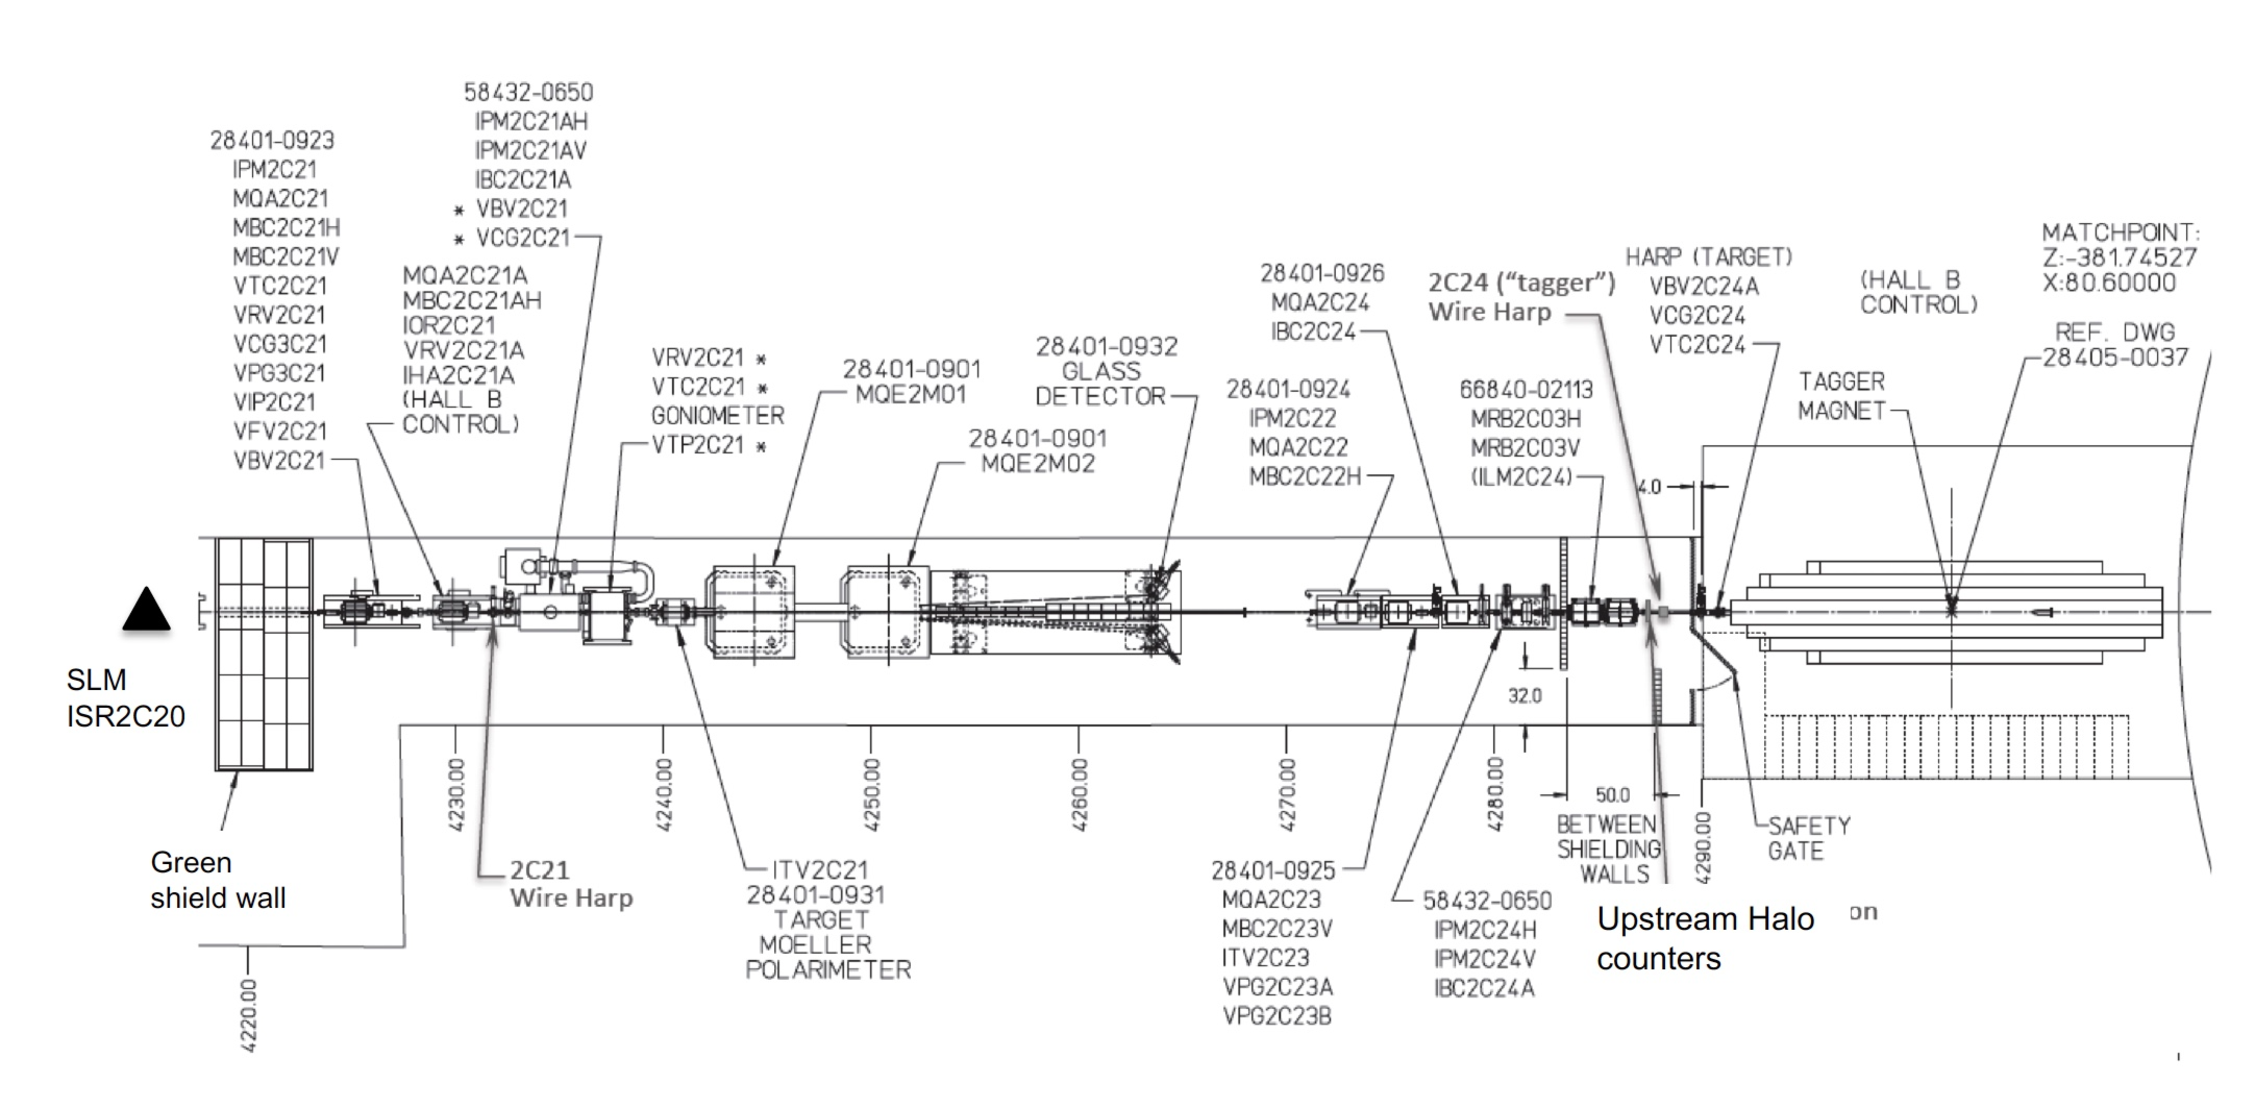
\includegraphics[width=1.\textwidth]{upstream_tunnel.pdf}
%\caption{Overhead view of the 2C beamline in the tunnel upstream of Hall B. {\color{red} Not the final figure.}}
%\label{fig:upstream}
%\end{center}
%\end{figure*}

 
This paper will discuss the design of the Hall-B beamline for CLAS12, and its performance during the 2018 experimental run. It will review the 
beamline instrumentation used to measure and monitor beam parameters and to protect CLAS12 detectors against errant beam motion. As will 
be demonstrated, excellent quality and stability of the CEBAF beams, coupled with the Hall-B beamline protection systems, allowed running the 
CLAS12 detector at the design luminosity.





\section{Hall-B Beamline Design}
\label{beamlinedesign}

As was described in Ref.~\cite{HPSBeamline}, the Hall B beamline is divided into two segments, the so-called ``2C" line from the Beam 
Switch Yard (BSY) following beam extraction from the CEBAF accelerator to the hall proper, and the ``2H" line from the upstream end of 
the experimental hall to the beam dump in the downstream tunnel. The beamline upstream of CLAS12 is furnished with a number of 
quadrupoles, corrector dipoles, and beam diagnostic tools, grouped into sections. Accelerator operators have exclusive control of these 
devices and use this instrumentation to tune and deliver the beam to the CLAS12 target located approximately at the geometrical center of the 
hall. In addition to the devices used by accelerator operations, there are several beam position, current, polarization, and halo monitors that 
are controlled and monitored by Hall-B shift personnel. 

For high-energy operation of CLAS12, the 2C beamline as described in Ref.~\cite{HPSBeamline} was modified to include 
the M{\o}ller polarimeter located in the upstream tunnel of the hall %(see Fig.~\ref{fig:upstream})
 and an intermediate beam dump just upstream 
of the hall. Additionally, the 2H beamline (Fig.~\ref{fig:hall1}) now includes a cryogenic target and a tungsten shield downstream of the 
target inside the CLAS12 torus magnet bore. The M{\o}ller polarimeter is used to periodically measure the longitudinal beam polarization and is discussed in more detail in Sec.~\ref{mollerpol}.  The other components are discussed immediately below.

% had to move this figure to intro section so that it would end up where I wanted it
%\begin{figure*}[t]
%\begin{center}
%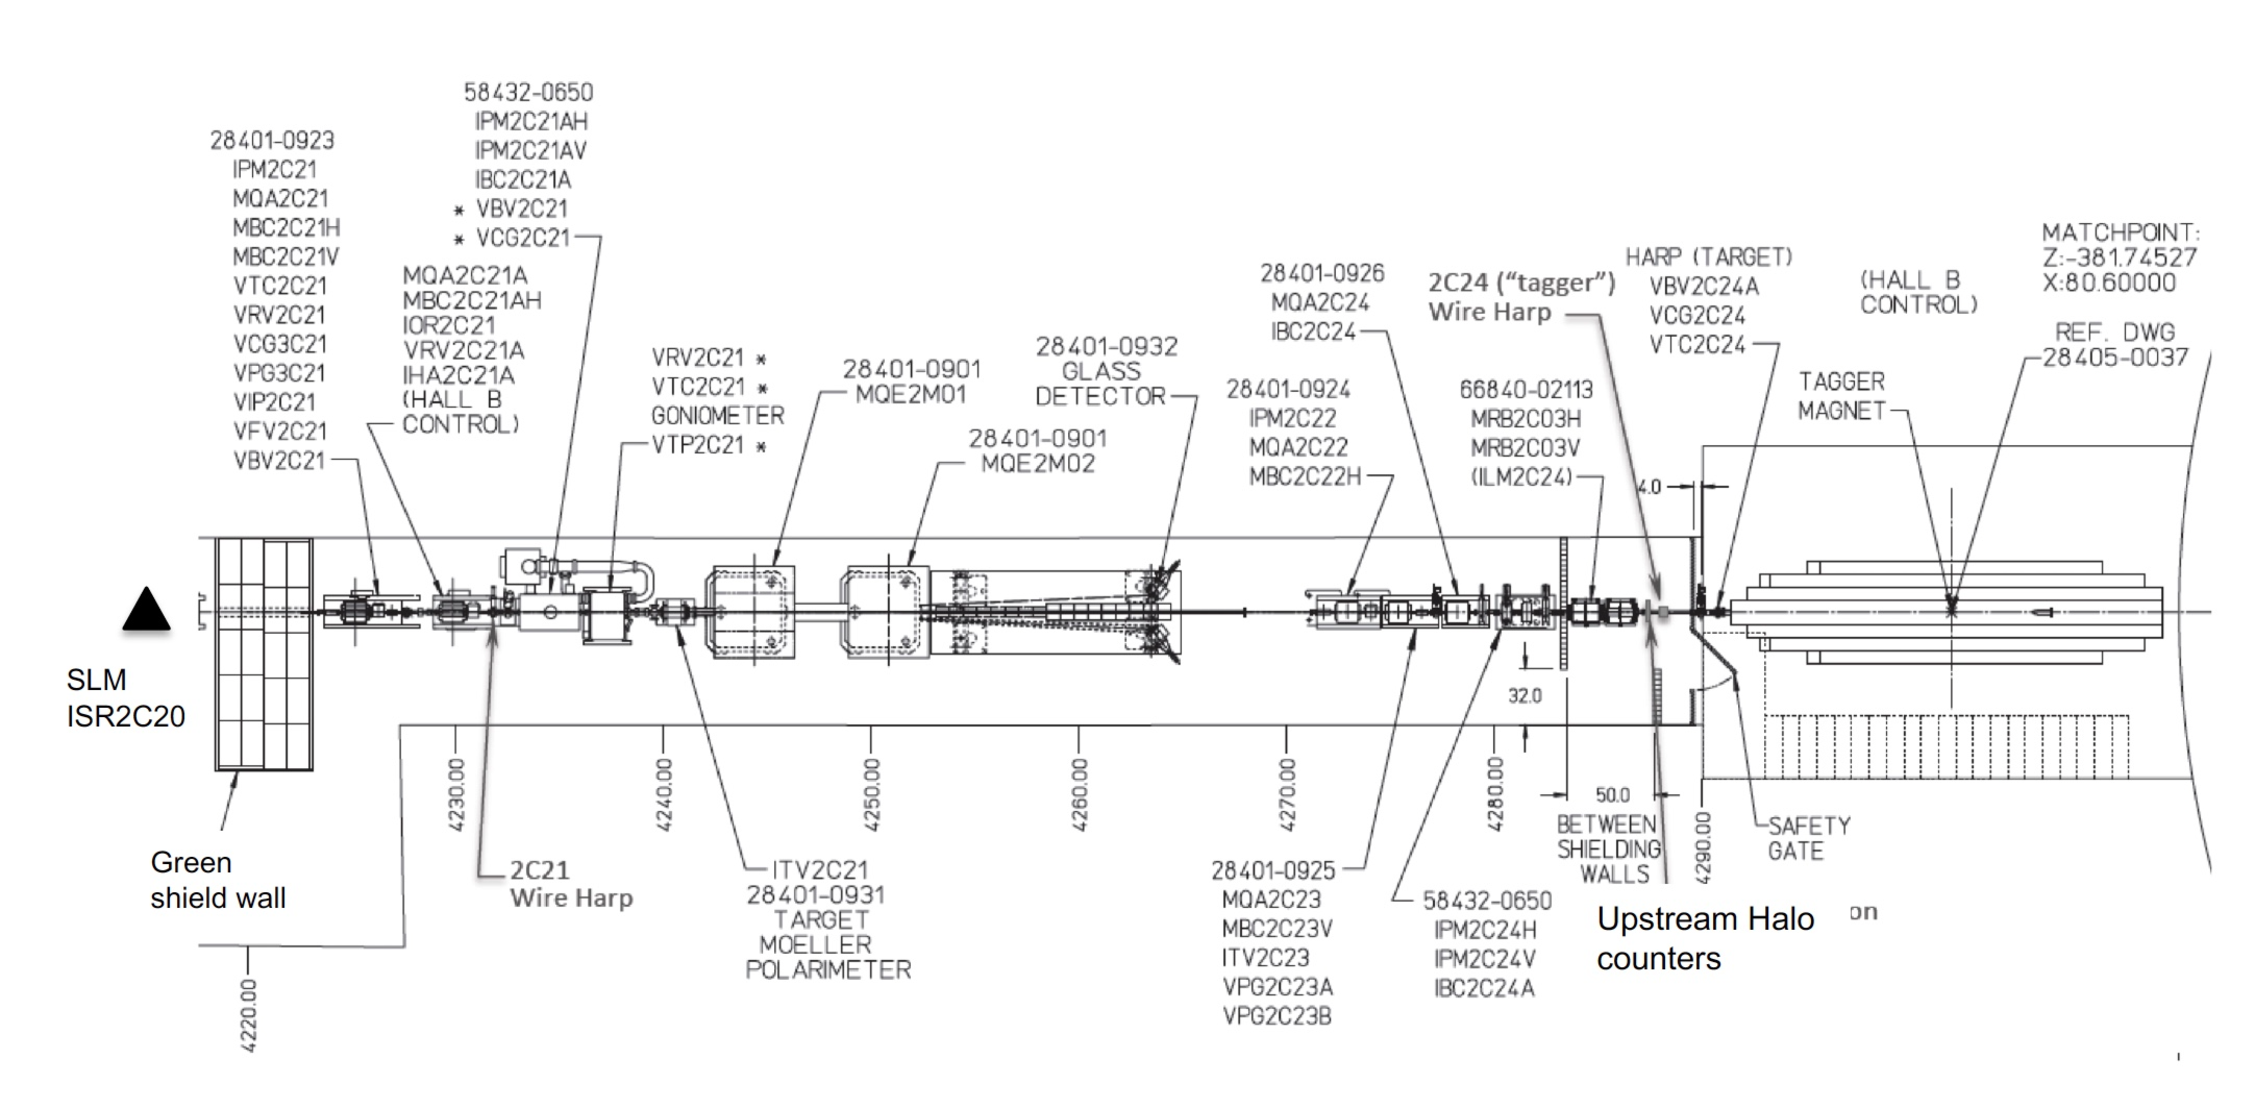
\includegraphics[width=1.\textwidth]{upstream_tunnel.pdf}
%\caption{Overhead view of the 2C beamline in the tunnel upstream of Hall B. {\color{red} Not the final figure.}}
%\label{fig:upstream}
%\end{center}
%\end{figure*}

\begin{figure*}[t]
\begin{center}
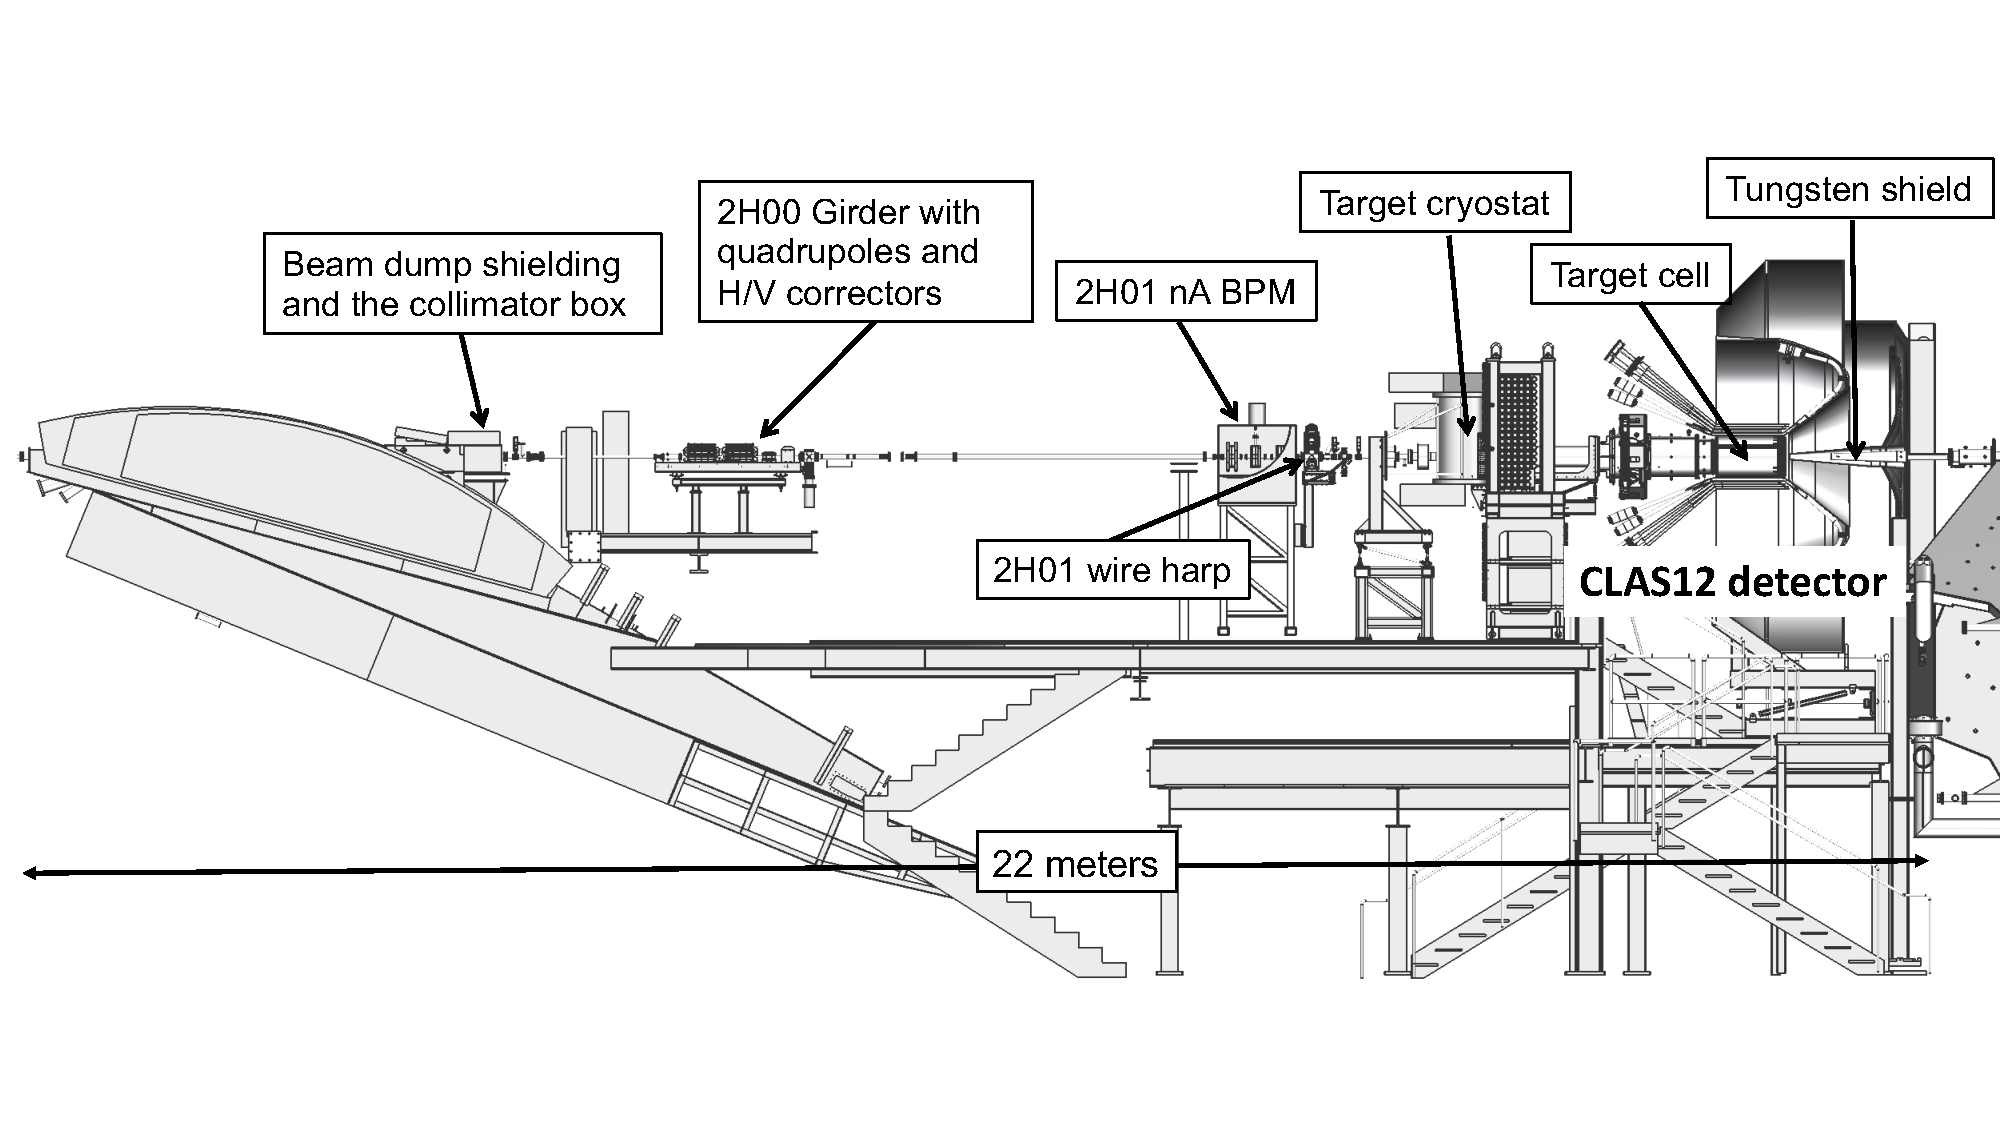
\includegraphics[width=1.\textwidth]{beamline_hall_1.pdf}
	\caption{Beamline in Hall B showing beamline elements upstream of the CLAS12 target, cryotarget, CLAS12 central detector and 
	the tungstem shield downstream of the scattering chamber.}
\label{fig:hall1}
\end{center}
\end{figure*}


\subsection{Intermediate beam dump before CLAS12}
\label{sec-IBD}

In order to prevent radiation damage to the sensitive detectors during the initial beam tune, or when errant beam may be sent to the hall, 
or during the beam polarization measurements with the M{\o}ller polarimeter, the beam has to be terminated upstream of CLAS12. For these 
operations the Hall-B tagger dipole magnet is used to deflect the primary beam and secondary scattering products. During low-energy 
operations, the tagger dipole directs the beam into the tagger beam dump in the hall floor upstream of the CLAS12 spectrometer. The highest 
energy beam that can be directed to this dump is limited to $6.2$ GeV by the maximum field of the tagger dipole, 
1.76 T \cite{tagger}. At higher energies, a few options for the intermediate beam dump were considered during the design stage with 
the optimal solution being to dump the beam inside the bore of the tagger magnet yoke. The design of the intermediate dump was based on
full FLUKA \cite{fluka} simulations and on thermal finite-element analysis. The two main parameters that were studied were the radiation levels at 
the location of the CLAS12 tracking detectors and the temperature rise in the magnet yoke when up to 10 nA of continuous wave (CW) 
electron beam is dumped on the yoke.  

The FLUKA simulations were used to determine background radiation levels at the tracking detectors for different configurations of the 
dump and compared with radiation levels from various targets and beam currents at the design luminosity.  It was found that acceptable 
background radiation levels from the dump occur when the beam is steered into the yoke at approximately 33 cm from the upstream 
entrance to the tagger magnet bore, as shown in Fig.~\ref{fig:yokedump}. This is done by setting the tagger magnetic field to be 
$I({\rm A}) = 43.491\times E({\rm GeV}) - 0.076$, where $I$ and $E$ are 
the tagger power supply current and the beam energy, respectively.   
%
\begin{figure}[hbt]
\begin{center}
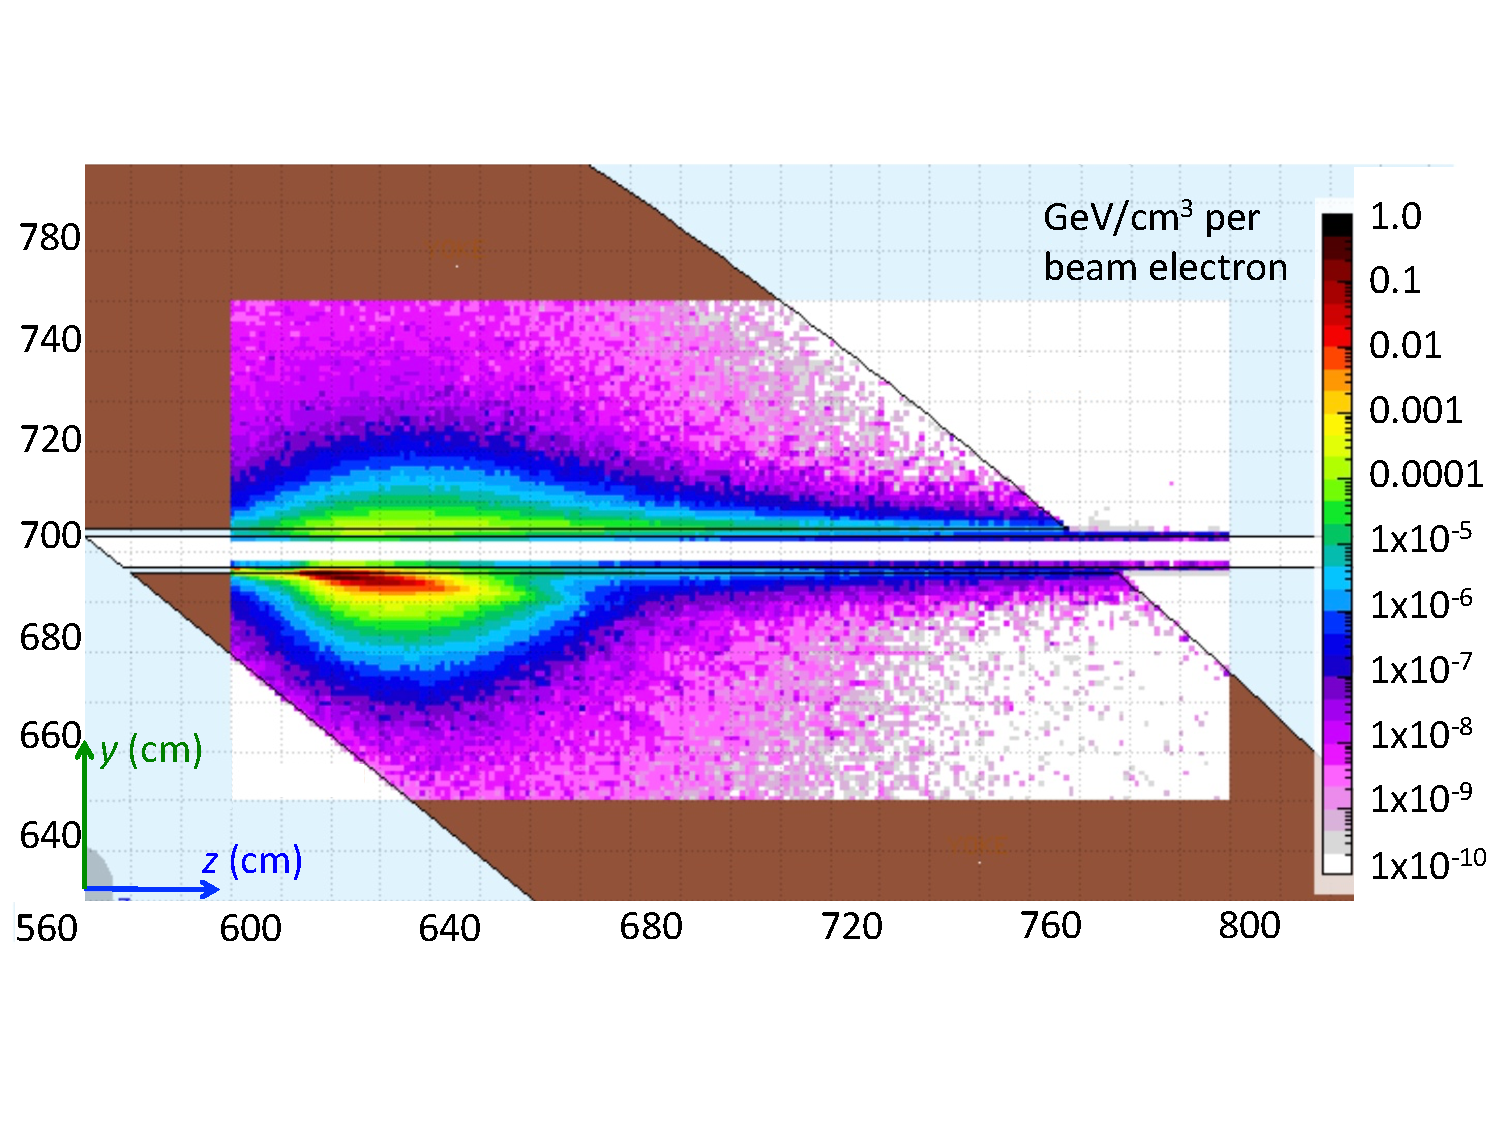
\includegraphics[width=.45\textwidth]{YokeDump.pdf}
	\caption{Distribution of energy in the yoke of the tagger dipole magnet from dumping a 10 nA, 11 GeV beam on the yoke at 
	$\sim33$ cm from the upstream entrance to the bore of tagger. Horizontal and vertical scales are distances in cm and energy 
	deposition (in GeV/cm$^3$) is indicated by the color scale. The brown region indicates the cross section of the tagger yoke.}
\label{fig:yokedump}
\end{center}
\end{figure}

The FLUKA simulations were also used to guide the design of the shielding around and just downstream of the tagger magnet yoke. 
The shielding includes lead, borated polyethylene, and concrete blocks. Figure~\ref{fig:raddem} shows the 1-MeV neutron equivalent 
fluency for the background from the dump and for various beam/target configurations as a function of the position along the beamline. 
In the graph, the yoke dump position is at approximately -900 cm and the CLAS12 target is at $\sim400$ cm. The figure shows that at 
the location of the CLAS12 target, the designed shielding configuration (green points) results in radiation levels from the yoke 
comparable to levels for running on a carbon target at the full design luminosity.   

\begin{figure}[hbt]
\begin{center}
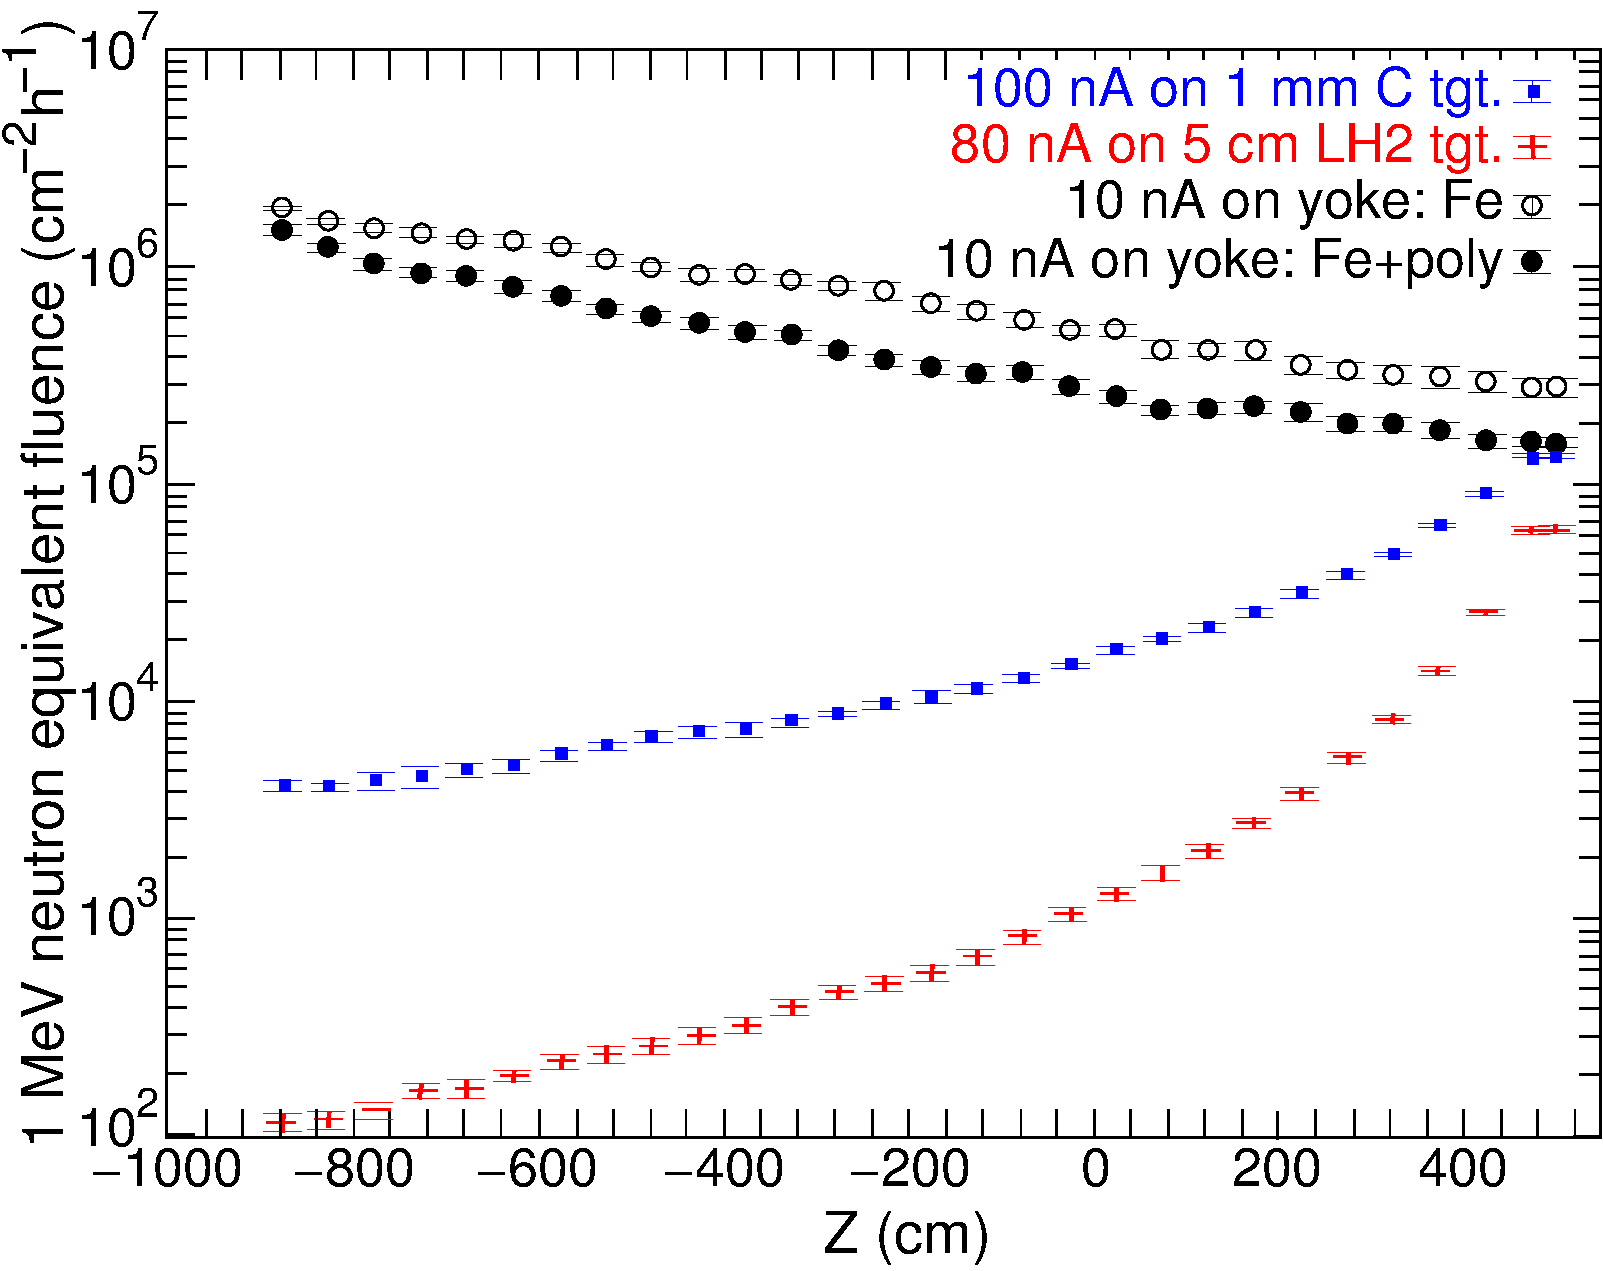
\includegraphics[width=0.45\textwidth]{Radiation.pdf}
%\includegraphics[width=0.45\textwidth]{radiation_hadrons.pdf}
	\caption{FLUKA simulation of radiation levels in the hall from dumping a 10 nA, 11 GeV beam on the tagger magnet yoke compared to 
	the radiation levels from nominal running on hydrogen and carbon targets. }
\label{fig:raddem}
\end{center}
\end{figure}

To assess the temperature increase in the yoke, a thermal finite-element analysis was set up using ANSYS Workbench v18 \cite{ANSYS}. 
A simplified CAD model of the yoke was imported and modified to include a cylindrical heat load representing the beam. The heating 
profile from the deposition of 1 kW of power in a cylinder of one Moliere radius ($r = 1.7$ cm) and 10 radiation lengths (17 cm) of iron 
was calculated. Conservatively, adiabatic boundary conditions were applied to the outer surfaces of the yoke. The model was solved as 
a transient thermal analysis with 100 time points over 3600 seconds. At the dump location, the temperature was found to initially increase
rapidly and then stabilized to a maximum temperature increase of $\Delta T = 54^\circ$C as the heat dissipates throughout the yoke 
volume (see Fig.~\ref{fig:ansys_yoke}). Due to the very large volume and heat capacity of the yoke, the temperature is not expected to 
rise much higher even for longer beam application times.

\begin{figure}[hbt]
\begin{center}
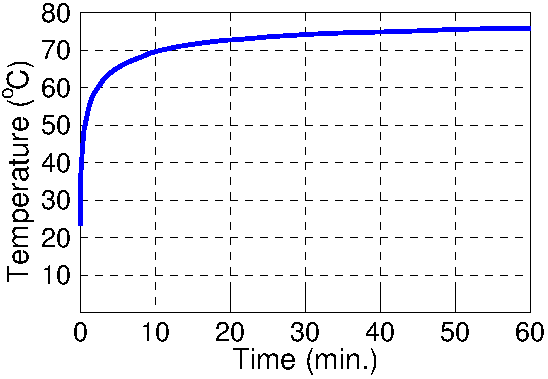
\includegraphics[width=0.45\textwidth]{YokeHeating.pdf}
	\caption{The heat distribution after $60$ minutes of beam exposure at the upstream dump location is shown. The highest 
	temperature in the yoke is at the region of the impact and is $76^\circ$C assuming an initial uniform temperature of $22^\circ$C.}
\label{fig:ansys_yoke}
\end{center}
\end{figure}





\subsection{Cryogenic target}
\label{sec-cryotgt}

Hall B experiments are grouped into running periods according to beam energy and targets. So far two types of cryogenic targets have been 
used for experiments; liquid hydrogen (LH$_2$) and liquid deuterium (LD$_2$). The Hall-B cryotarget system from the $6$ GeV era  
\cite{CLAS} has been modified for CLAS12 operation.  The current target cell is a 20-mm diameter, 50-mm long Kapton cylinder
with 10-mm-diameter, and 30-$\mu$m-thick aluminum entrance and exit windows. The typical target density is $71$ mg/cm$^3$ for LH$_2$ 
and $169$ mg/cm$^3$ for LD$_2$. Figure~\ref{fig:targsch} shows the design 
rendering of the target cell inside the scattering chamber.  The scattering chamber is made of Rohacell XT110 foam (density 
$\rho=0.110$ g/cm$^3$) and is $\sim$45 cm long with a 100 mm outer diameter such that it fits within the CLAS12 silicon tracker (SVT) 
(described elsewhere in this volume) and provides a minimal material thickness for scattered particles from the target to the CLAS12 detectors.  

A beam halo monitor is integrated within the target cell. This device consists of a 40-mm-long glass cylinder with inner and outer diameters 
of 10 mm and 12 mm, respectively, mounted directly on the upstream window of the target cell with its axis parallel to the beamline and 
with 16 optical fibers attached to the upstream perimeter of the cylinder. Light generated in the cylinder 
from interactions of the beam halo or from back-scattered secondaries are readout with a multi-anode photomultiplier tube. The device, called 
the  beam-offset monitor (BOM), is used to monitor the beam position at the target (see discussion below).  

The scattering chamber extends downstream of the Central Detector. There is a 50-$\mu$m-thick aluminum window on the downstream end 
of the scattering chamber that closes the upstream vacuum beamline (from the accelerator to the CLAS12 target). The downstream vacuum 
beamline starts after a 60-cm-long air gap after the scattering chamber and ends at the beam dump.  

\begin{figure}[t]
\begin{center}
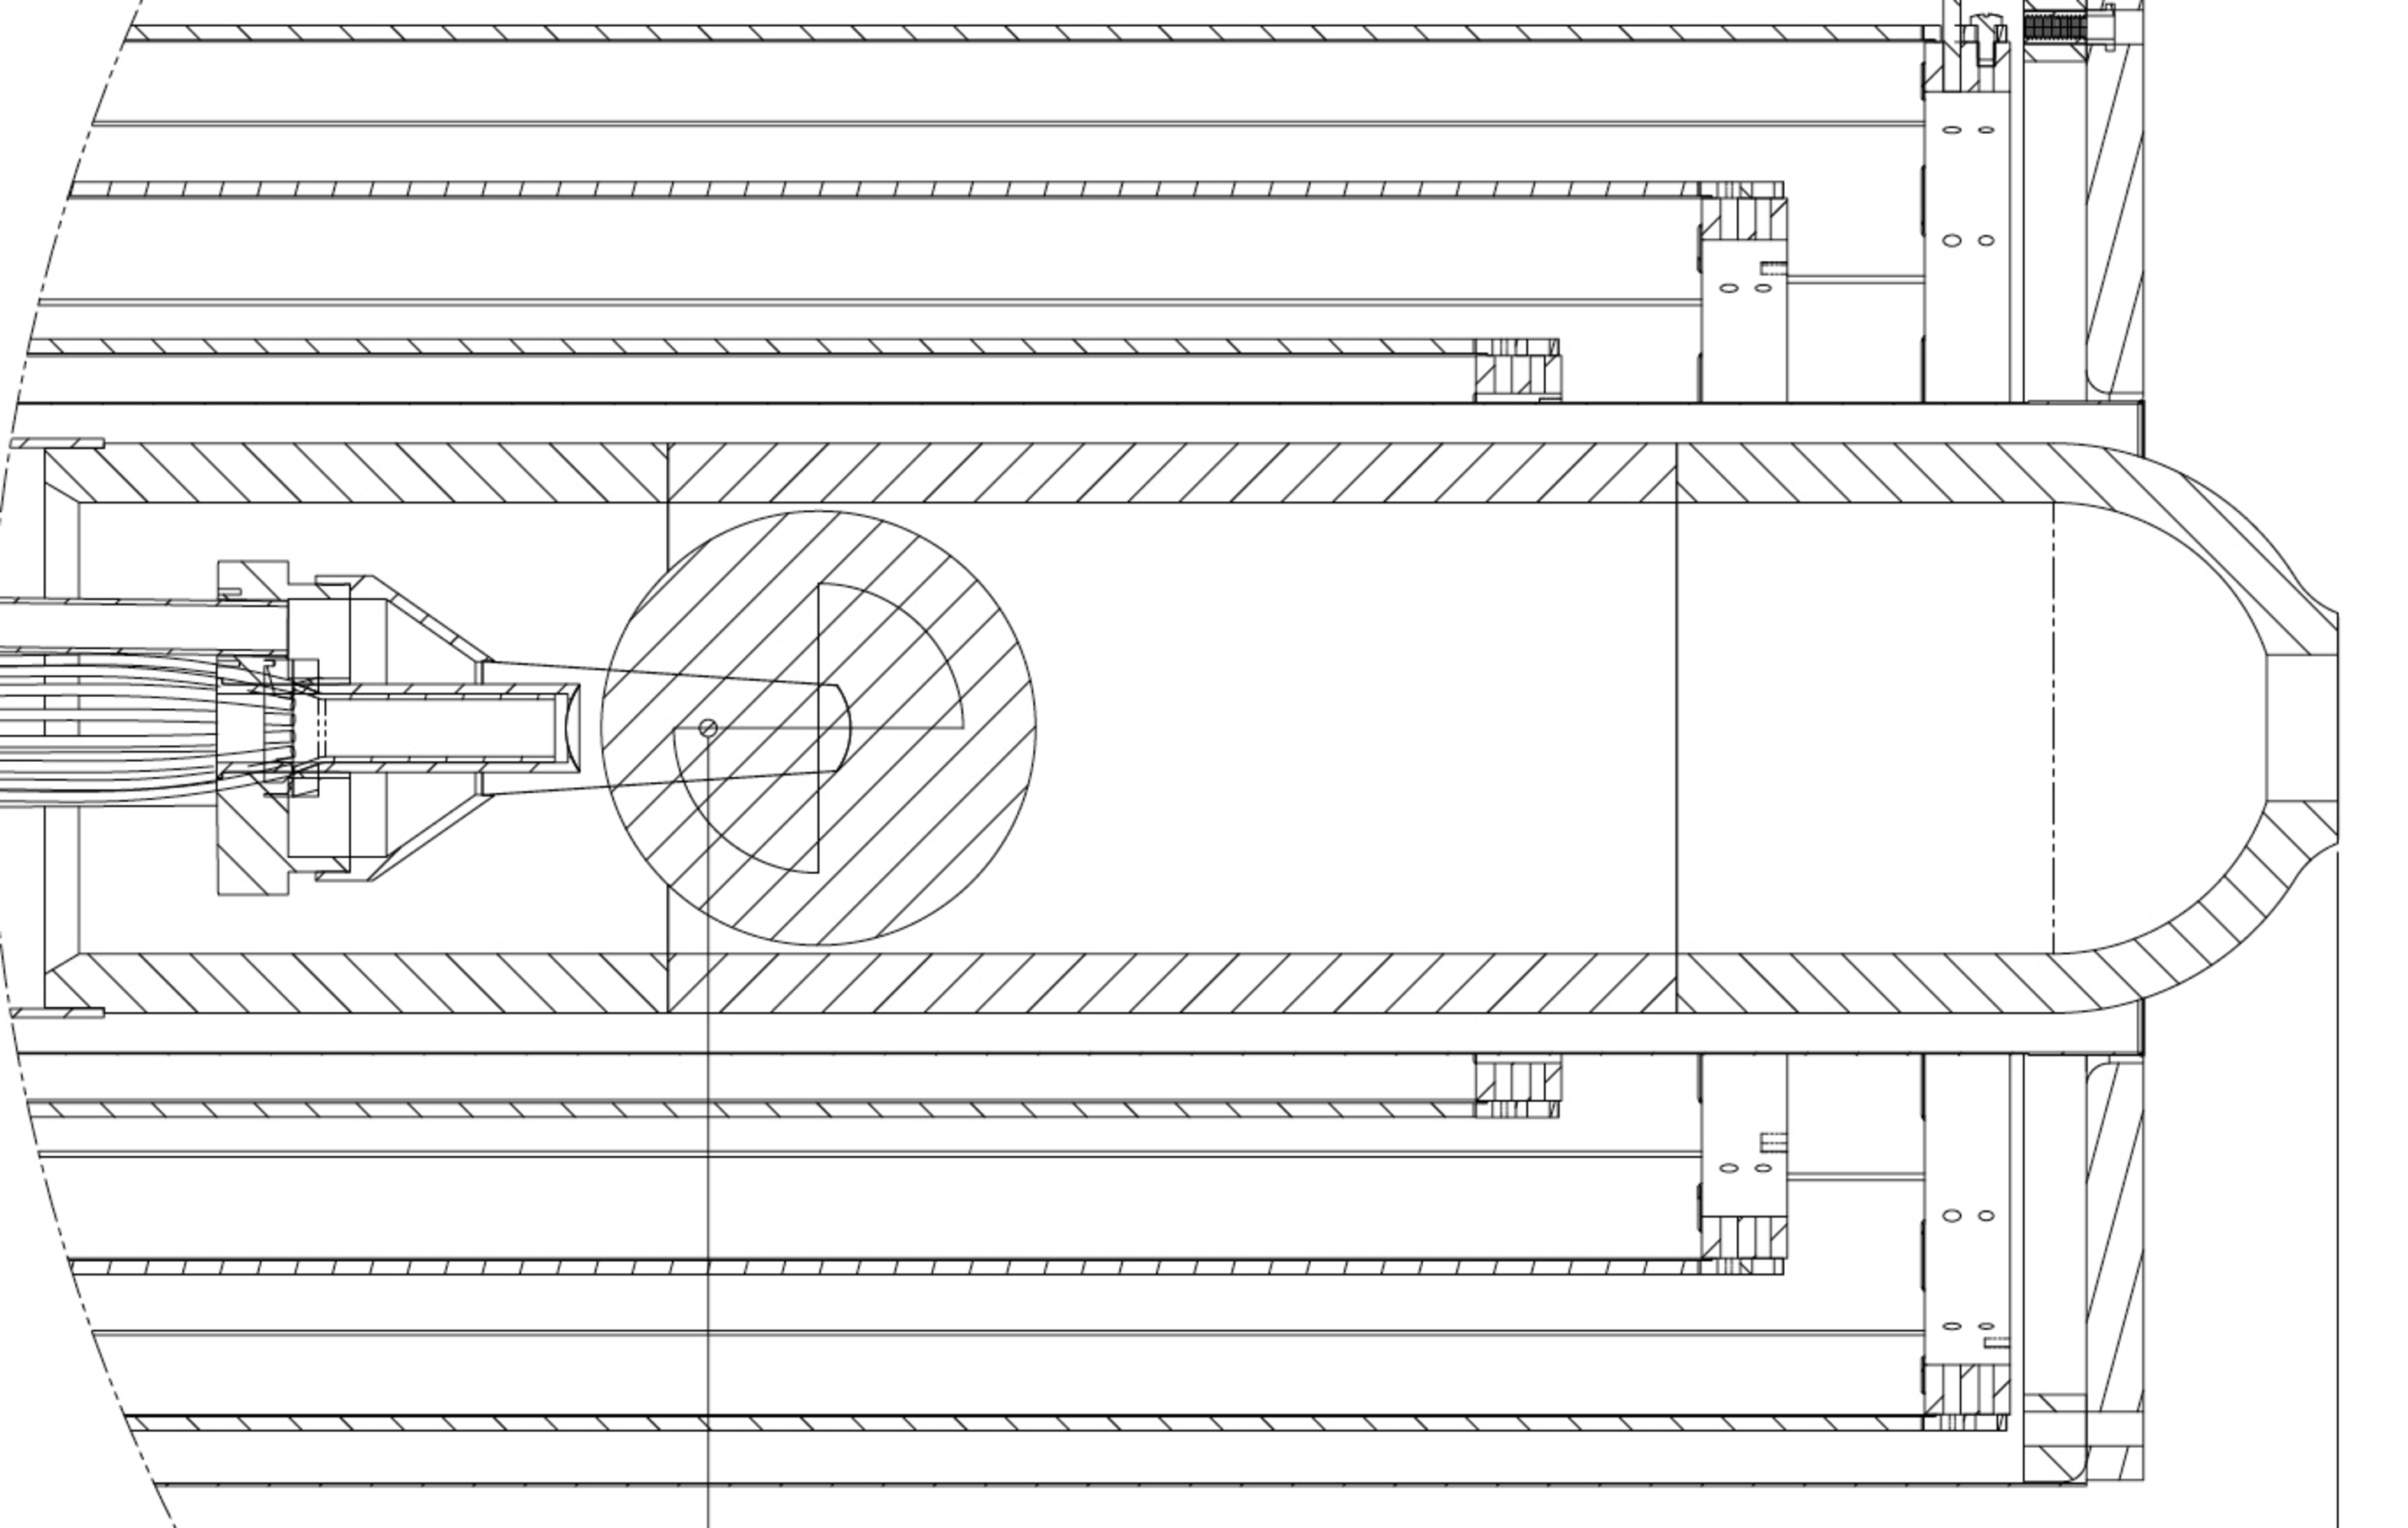
\includegraphics[width=0.45\textwidth]{target_sch.pdf}
%\includegraphics[width=0.45\textwidth]{TCell.pdf}
	\caption{Sketch of the cryogenic target showing the target cell, beam offset monitor, and scattering chamber with associated plumbing 
	and structural supports.}
\label{fig:targsch}
\end{center}
\end{figure}

\begin{figure*}[t]
\begin{center}
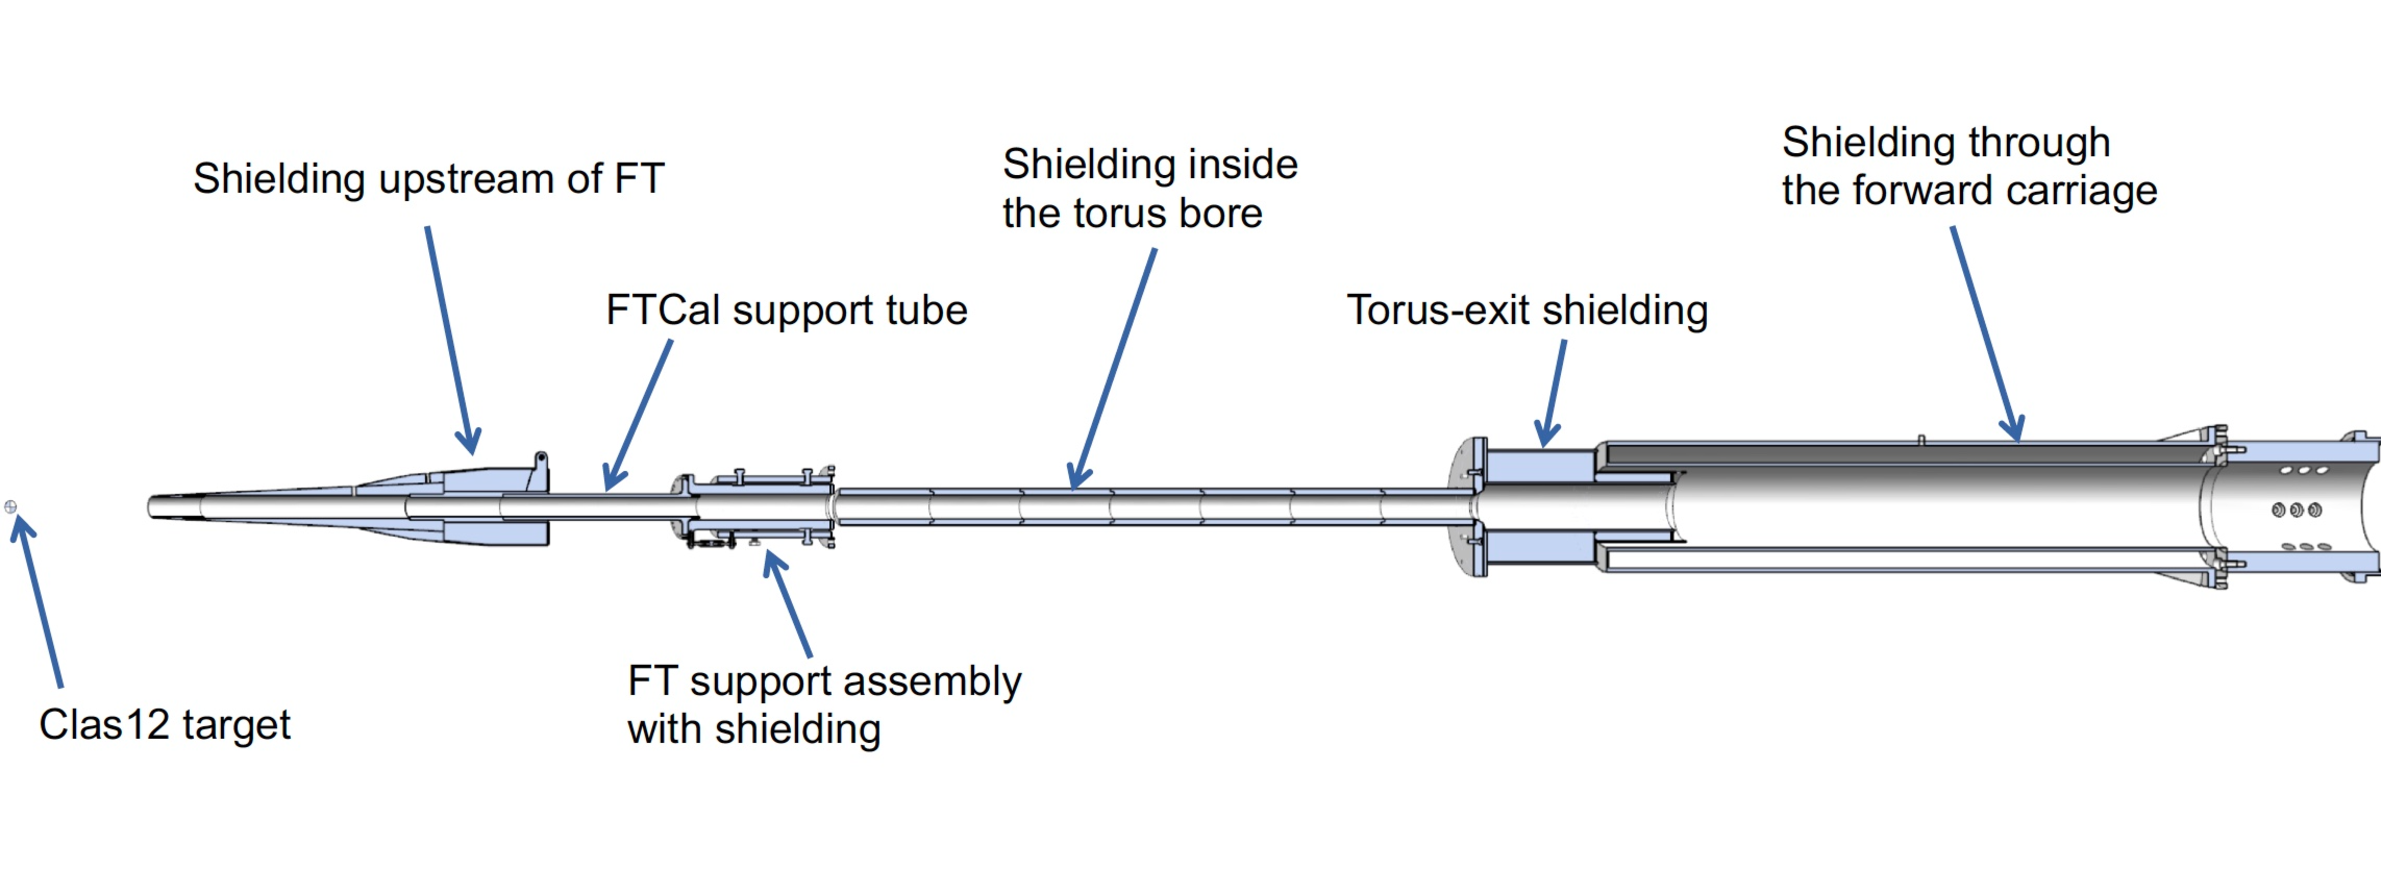
\includegraphics[width=1.\textwidth]{beamline_hall_shielding.pdf}
\caption{Tungsten shielding downstream of the target, through the torus magnet bore.}
\label{fig:shield}
\end{center}
\end{figure*}


In addition to the cryogenic targets mentioned above and already used in two experiments (LH$_2$ and LD$_2$), there will be experiments
that will use nuclear targets in the form of thin foils and experiments with polarized targets. The nuclear target assembly is similar to the 
cryogenic target cell except that various target foils will be inside the cell instead of a liquid. The cryotarget supply lines will be used to flow 
helium gas through the cell to dissipate heat in the foils from the beam. Two types of polarized targets will be used for CLAS12 experiments
\cite{Keith:2015ete}; dynamically (longitudinally) polarized ammonia (NH$_3$) and deuterated ammonia (ND$_3$), and a polarized solid 
HD target in a frozen spin mode. 

\subsection{Shielding downstream of the target} 

Special care was taken to protect the CLAS12 detectors from beam-induced background radiation. The main sources of the background are 
small-angle electron scattering along with electromagnetic processes such as bremsstrahlung, pair production, and M{\o}ller scattering. 
These interactions produce photons, electrons, and positrons that can flood the tracking detectors. GEANT4 simulations of CLAS12
have been used to study backgrounds and design appropriate shielding to reduce the levels of background radiation.  The shielding design
takes advantage of the 5-T longitudinal magnetic field around the target that is generated by the Central Detector superconducting solenoid 
magnet. This strong longitudinal magnetic field causes low-energy particles to spiral forward and away from the detectors and into the 
shielding far downstream of the target. The heavy shielding materials (lead and tungsten) contain the background and either absorb it or 
guide the flux of particles out the downstream end of CLAS12 without interacting in the detectors. 

Because CLAS12 will run with and without the Forward Tagger (FT) (described elsewhere in this volume) in use, two shielding 
configurations were designed. Figure~\ref{fig:shield} shows the configuration when the FT is in use. The shielding starts with a 
tungsten cone with a 5-cm diameter hole at the center for the beam. When the FT is in use, the tungsten cone is mounted directly 
to the FT central support, which is also made from tungsten. In this case, the angular acceptance of particles scattered from the target 
starts at $\sim 2^\circ$. For the configuration without the FT, a large diameter lead cylinder is inserted between the FT central support 
(after removing the FT tracker) and the tungsten cone, thus moving the cone closer to the target. In this case the acceptance for forward 
scattered particles starts at $\sim 5^\circ$. The shielding elements also include cylindrical tungsten absorbers inside the torus bore, a 
tungsten shield around the FT mounting fixture to the torus, and a lead-tungsten shield downstream of the torus.  

\begin{figure}[t]
\begin{center}
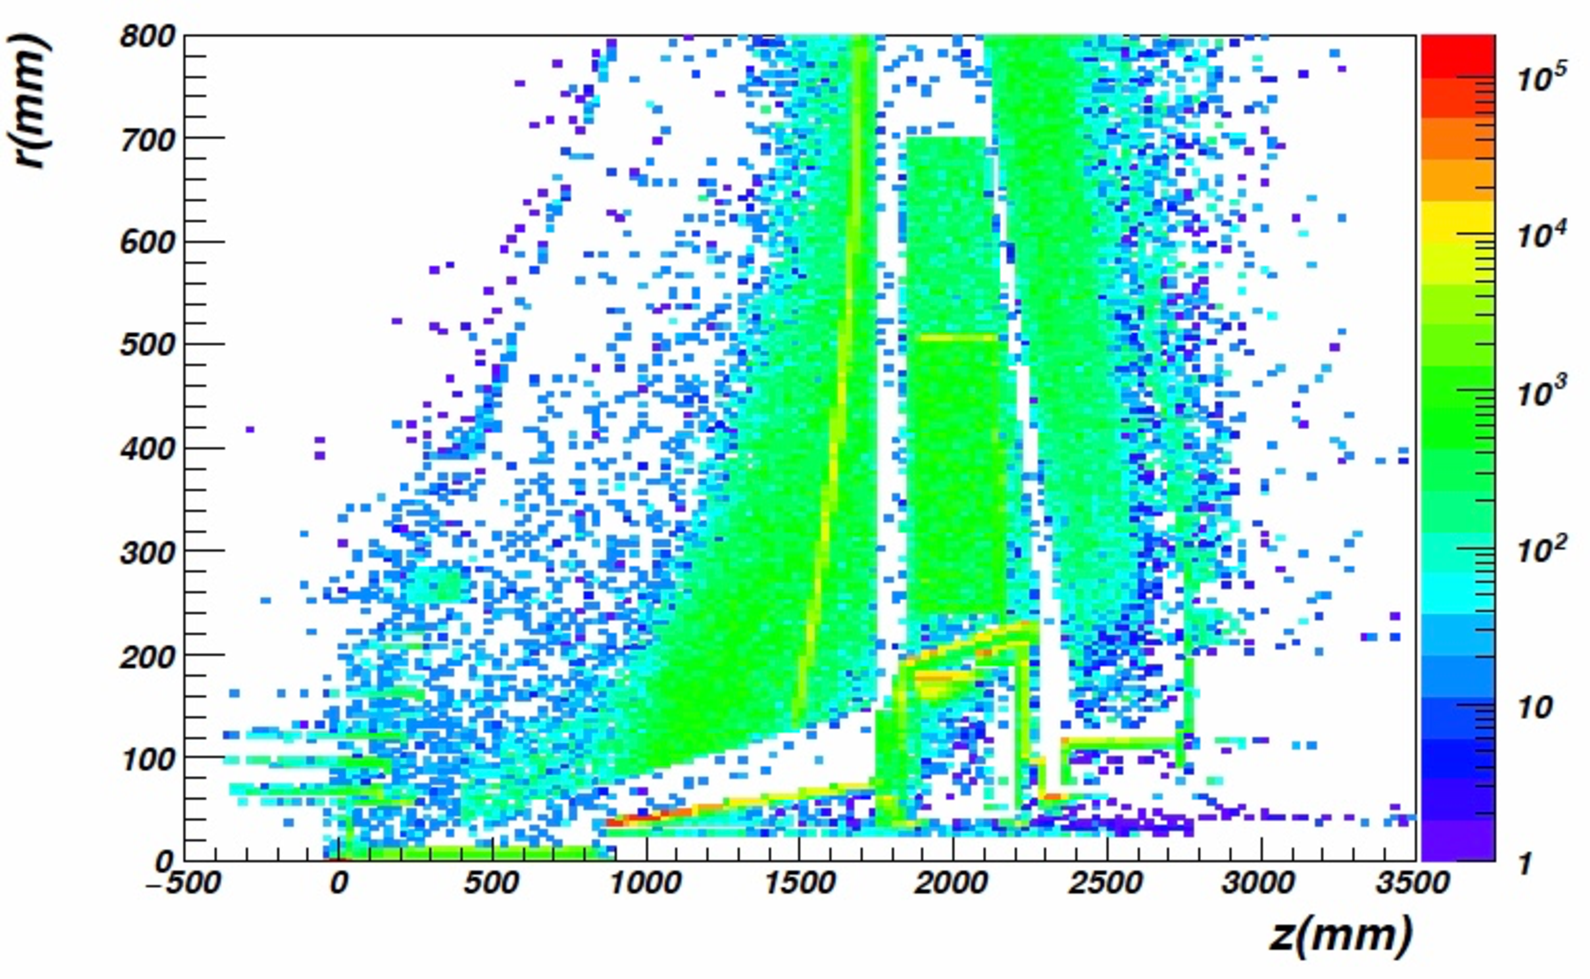
\includegraphics[width=0.48\textwidth]{fton_final_origin.pdf}
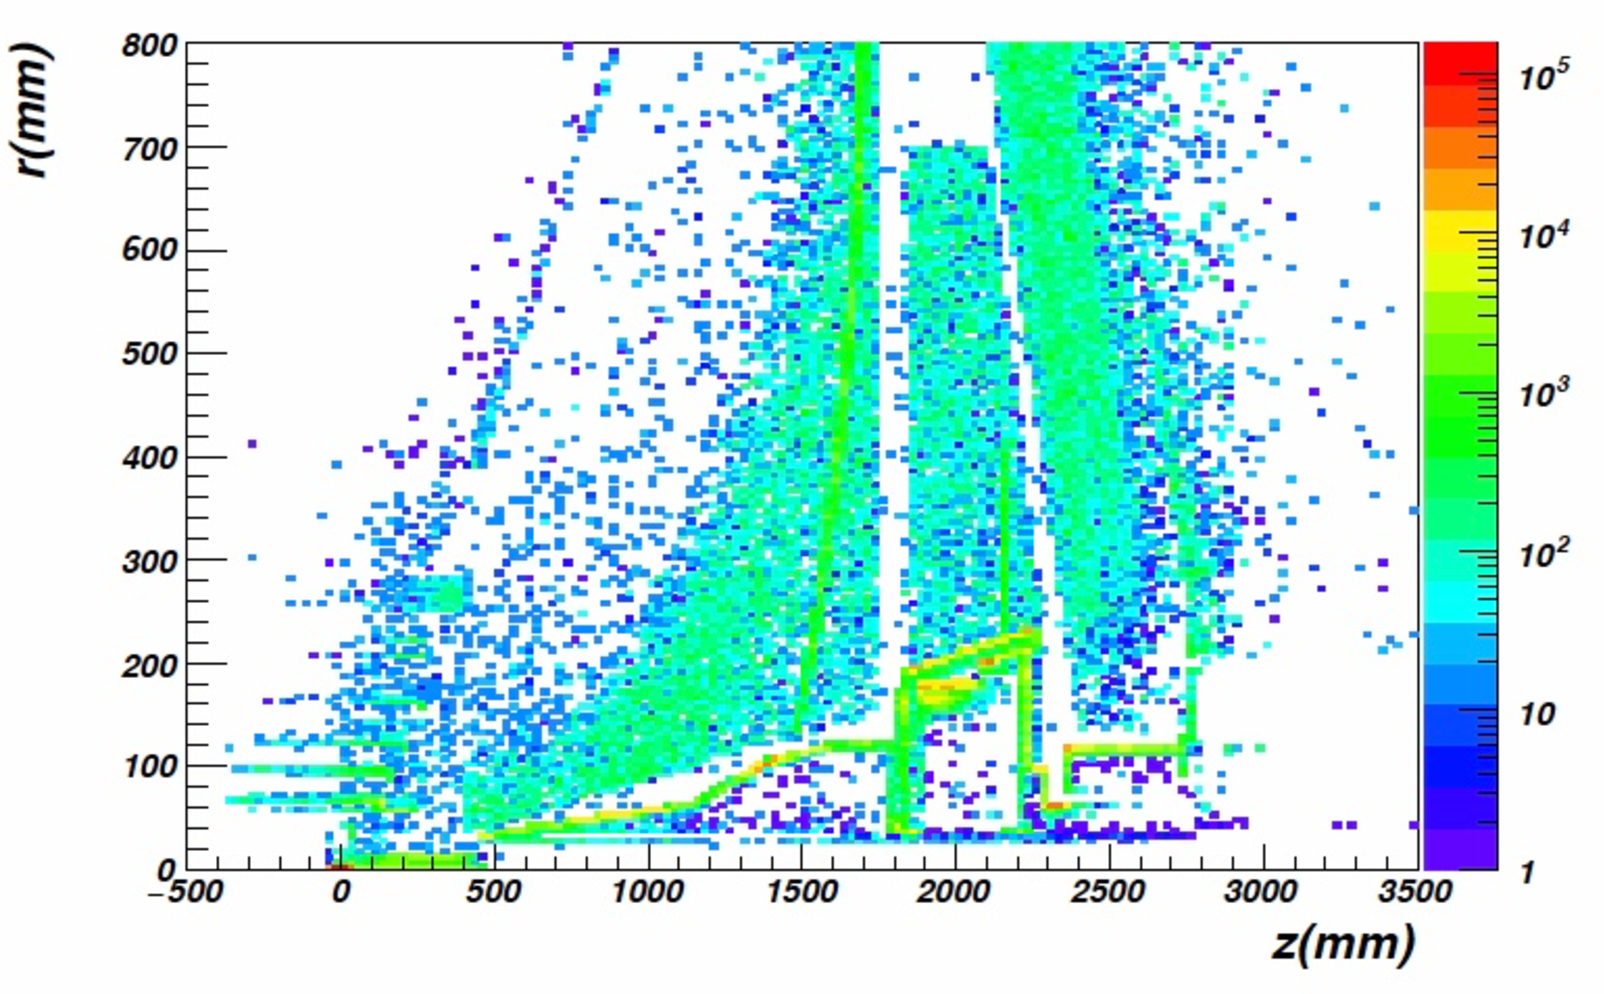
\includegraphics[width=0.48\textwidth]{ftoff_final_origin.pdf}
	\caption{The origin of particles hitting Region 1 drift chambers in the $R$-$z$ plane, where $R$ is the transverse distance from 
	the beam and the $z$ is in the beam direction. The top graph corresponds to the FT-on configuration and the bottom graph is for 
	FT-off. The main source of the background is the target located at $R=0$ and $z=0$. The second largest source is the edge of 
	the tungsten shield that starts from (40,850) and extends to (60,1700), followed by the outer edge of the Forward Tagger calorimeter 
	enclosure located around $R=200$ mm and $z=2000$ mm. The other large source is the mirror of the high-threshold Cherenkov 
	counter shown as almost vertical band at around $z=1550$ mm.}
\label{fig:origin}
\end{center}
\end{figure}

One of the main criteria for the shielding design is to maintain an occupancy rate in the drift chambers (described elsewhere in this volume)
of less than 4\% since higher occupancies adversely affect the track reconstruction efficiency.  Drift chamber occupancies were simulated 
by accumulating hits in the detector elements over 250-ns time frames, which roughly corresponds to the time readout window for the drift 
chambers. The simulated beam was spread out over this time window to match the actual beam structure and was incident on the 5-cm-long 
LH$_2$ target such that the design luminosity of $10^{35}$ cm$^{-2}$ s$^{-1}$ was achieved in the simulation. The simulated target 
included the aluminum entrance and exit foils and the air gap downstream of the target. The final shielding configuration resulted in 
occupancies of less than about 3\% for the FT-on configuration and less than about 1.5\% for the FT-off configuration.  Figure~\ref{fig:origin} 
shows the origins of background particles hitting the drift chambers for both shielding configurations. The main source of the background 
is the target with other sources being the edges of the tungsten shield, and detector enclosures (see figure caption for details). 




\section{Performance}The HTCC is one of the major CLAS12 systems used in experiments with the electron beam. The most important aspects of the HTCC performance are that it provides good timing, high electron detection efficiency, high signal strength, and high rejection factor of charged pions. All these parameters are critical for the quality of the data obtained in experiments since the detector, in combination with the forward calorimeter [ref. to ECAL], provides a fast trigger signal for CLAS12. As shown in section 6 the MC prediction for the HTCC for electrons is $\approx$100\%. Fig.~\ref{fig:RAFO_2GeV}. shows the experimentally measured electron detection efficiency for elastically scattered electrons at 2 GeV. The corresponding thresholds applied were approximately 2.5 photoelectrons. Measurements were performed using a special procedure with a random trigger that was not correlated with the HTCC. There were observed 27 events not detected by the HTCC due to the applied threshold. As shown, the electron detection efficiency is $\eta$ = (99$\pm$0.2)\%, which is in good agreement with the MC estimate. This result can be considered as a conservative estimate due to relatively high threshold used in measurements. Moreover, electrons travel a longer distance in the radiator gas (10 \% to 30 \% difference depending on a scattering angle). For these electrons the signal strength is higher, and therefore the detection efficiency is higher also as compared with the aforementioned efficiency for the elastically scattered electrons.   

\begin{figure}[!ht]
    \centering
    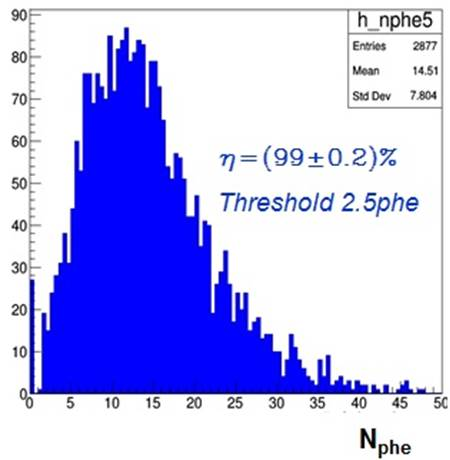
\includegraphics[width=1.0\linewidth,trim={0.0cm 0.0cm 0.0cm 0.0cm},clip]{images/RAFO_2GeV.jpg}
    \caption{Electron detection efficiency for elastically scattered electrons at 2 GeV. Data are obtained with the random trigger not correlated with the HTCC or other detector components of CLAS12.}
    \label{fig:RAFO_2GeV}
\end{figure}

Fig.~\ref{fig:positivePNPEC6595} shows the response of the detector in a wide range of particle momentum. The increase of number of events at high momenta is due to registration of charged pions (above threshold of their registration in the HTCC) and this is clearly illustrated.

\begin{figure}[!ht]
    \centering
    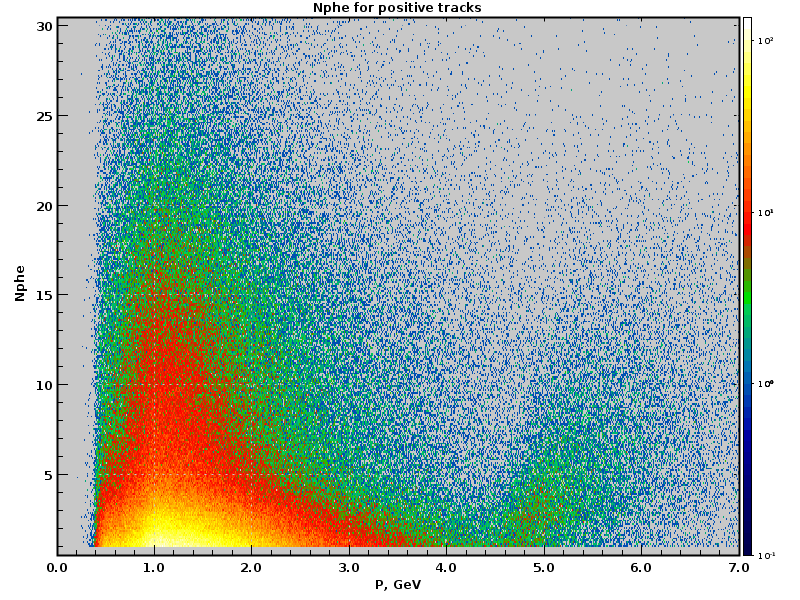
\includegraphics[width=1.0\linewidth,trim={0.0cm 0.0cm 0.0cm 0.0cm},clip]{images/positivePNPEC6595.png}
    \caption{Distributions of the HTCC response in a wide momentum range, including the region beyond the threshold of charged pion registration. Data obtained for positrons and $\pi^{+}$-mesons.}
    \label{fig:positivePNPEC6595}
\end{figure}

\begin{comment}
As shown bellow in the Fig.~\ref{fig:avgNPE_Theta_Phi_Dev_Build-2_NO_HOLES} the signal strength goes up for the utmost mirrors (large electron scattering angles). This is because electrons travel a longer distance in the radiator gas (10\% to 30\% difference depending on angle.) In other words the electron detection efficiency obtained for elastically scattered electrons at 2 GeV can be considered as as a conservative estimate for the efficiency of electron detection at larger angles.
\end{comment} 

The signal strength in the HTCC depends on the actual properties of the mirror facets, such as their final shape and reflectance. The accuracy of the combined mirror assembly and the alignment of the HTCC components (mirror, PMTs, Winston Cones), and the composition of the radiator gas all influence the final results. The FADC histogram of  the typical signal strength distribution obtained in one half-sector \#1 and \#2 of Sector 1 is shown in Fig.~\ref{fig:Signal_S1_HS1_HS2_R1_R2}. The signal strength for scattered electrons averaged over all HTCC channels is shown in Fig.~\ref{fig:Average_HTCC_Signal}. The experimentally measured mean value of 16.3 phe is close to Monte-Carlo simulation results, (see Fig.~\ref{fig:10cm_Targ_5T_Field_Phi}).

\begin{figure}[!ht]
    \centering
    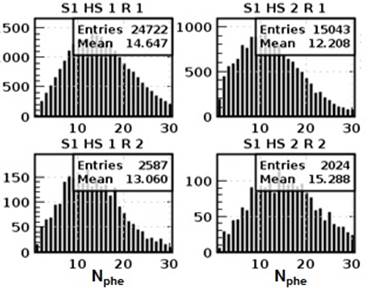
\includegraphics[width=1.0\linewidth,trim={0.0cm 0.0cm 0.0cm 0.0cm},clip]{images/Signal_S1_HS1_HS2_R1_R2.jpg}
    \caption{Typical distributions of the signal strength in channels covering polar angles in the range of $5^\circ$ to $12.5^\circ$ (Ring 1) and $12.5^\circ$ to $20.0^\circ$ (Ring 2) within azimuthal interval of $60^\circ$.}
    \label{fig:Signal_S1_HS1_HS2_R1_R2}
\end{figure}

\begin{figure}[!ht]
    \centering
    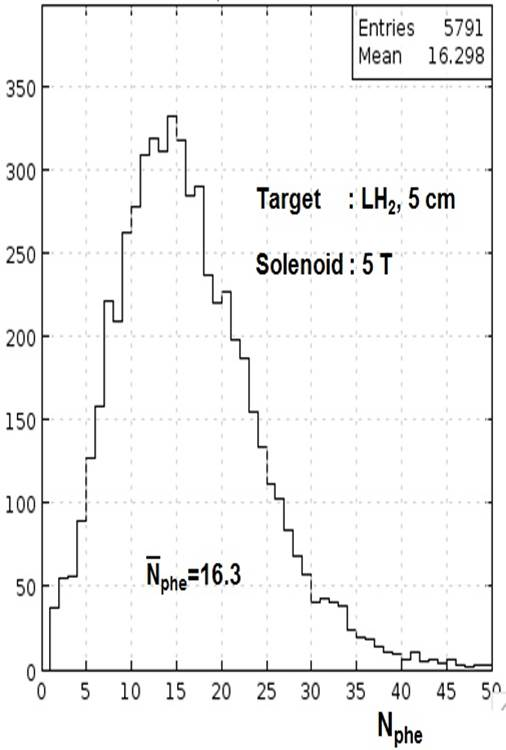
\includegraphics[width=1.0\linewidth,trim={0.0cm 0.0cm 0.0cm 0.0cm},clip]{images/Average_HTCC_Signal.jpg}
    \caption{The HTCC average signal strength for electrons from beam data.}
    \label{fig:Average_HTCC_Signal}
\end{figure}

Fig.~\ref{fig:HTCC_Response_run4013} shows the HTCC response for different electron momenta. Fig.~\ref{fig:avgNPE_Theta_Phi_Dev_Build-2_NO_HOLES}  shows the distribution of the HTCC response over the entire face of the mirror in the $x-y$-plane. Similar distribution is shown in Fig.~\ref{fig:avgNPE_XY_Dev_Build_02npe} obtained at the lower electron detection threshold of 0.2 photoelectrons. At the large electron scattering angles in range of 27.5$^\circ$ to 35$^\circ$, the statistics is lower. Fig.~\ref{fig:statistics_Theta_Phi_Dev_Build_NO_HOLES} shows the distribution of statistics in all 6 sectors. The data shows that the integrated signal strength is about 16.5 photoelectrons.

\begin{figure}[!ht]
    \centering
    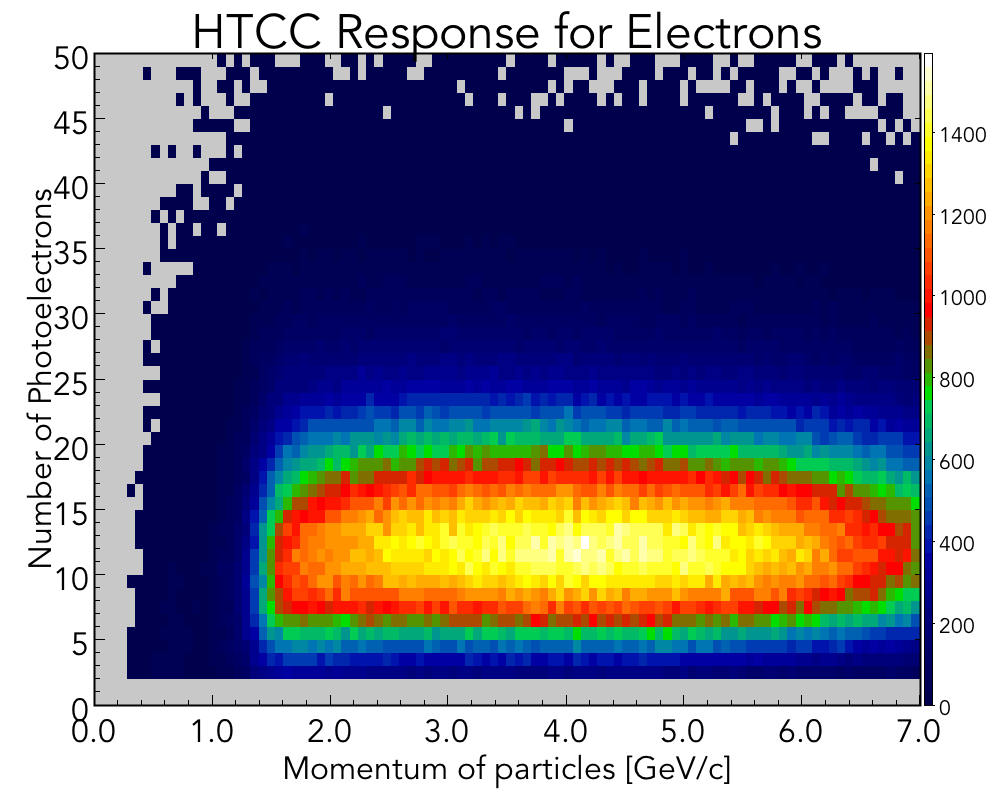
\includegraphics[width=1.0\linewidth,trim={0.0cm 0.0cm 0.0cm 1.73cm},clip]{images/HTCC_Response_run4013.png}
    \caption{The HTCC response for electrons: signal strength vs. momentum at 10.6 GeV energy.}
    \label{fig:HTCC_Response_run4013}
\end{figure}

\begin{figure}[!ht]
    \centering
    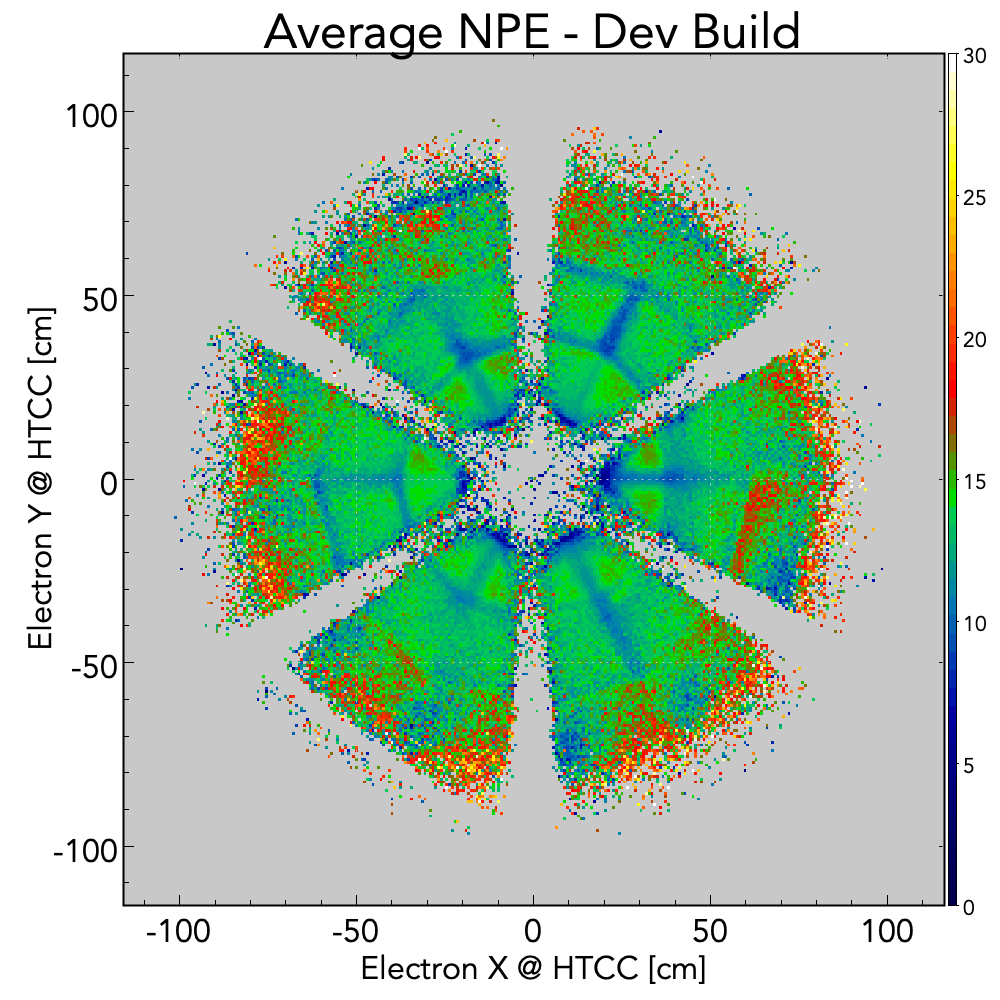
\includegraphics[width=1.0\linewidth,trim={0.0cm 0.0cm 0.0cm 1.67cm},clip]{images/avgNPE_Theta_Phi_Dev_Build-2_NO_HOLES.png}
    \caption{The HTCC response (in $N_{phe}$) for electrons in $x-y$-plane of the mirror.}
    \label{fig:avgNPE_Theta_Phi_Dev_Build-2_NO_HOLES}
\end{figure}

\begin{figure}[!ht]
    \centering
    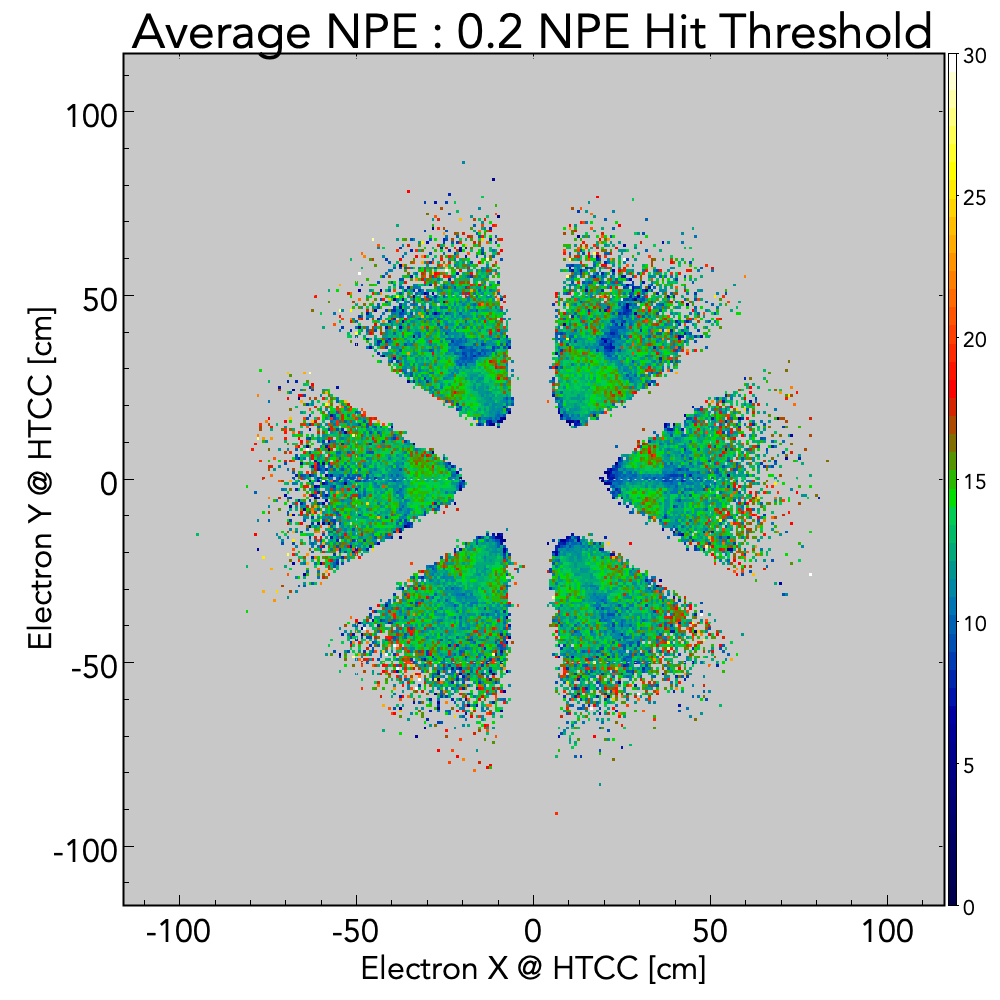
\includegraphics[width=1.0\linewidth,trim={0.0cm 0.0cm 0.0cm 1.67cm},clip]{images/avgNPE_XY_Dev_Build_02npe.png}
    \caption{The HTCC response (in $N_{phe}$) for electrons in $x-y$-plane of the mirror at the electron detection threshold of 0.2 photoelectrons.}
    \label{fig:avgNPE_XY_Dev_Build_02npe}
\end{figure}

\begin{figure}[!ht]
    \centering
    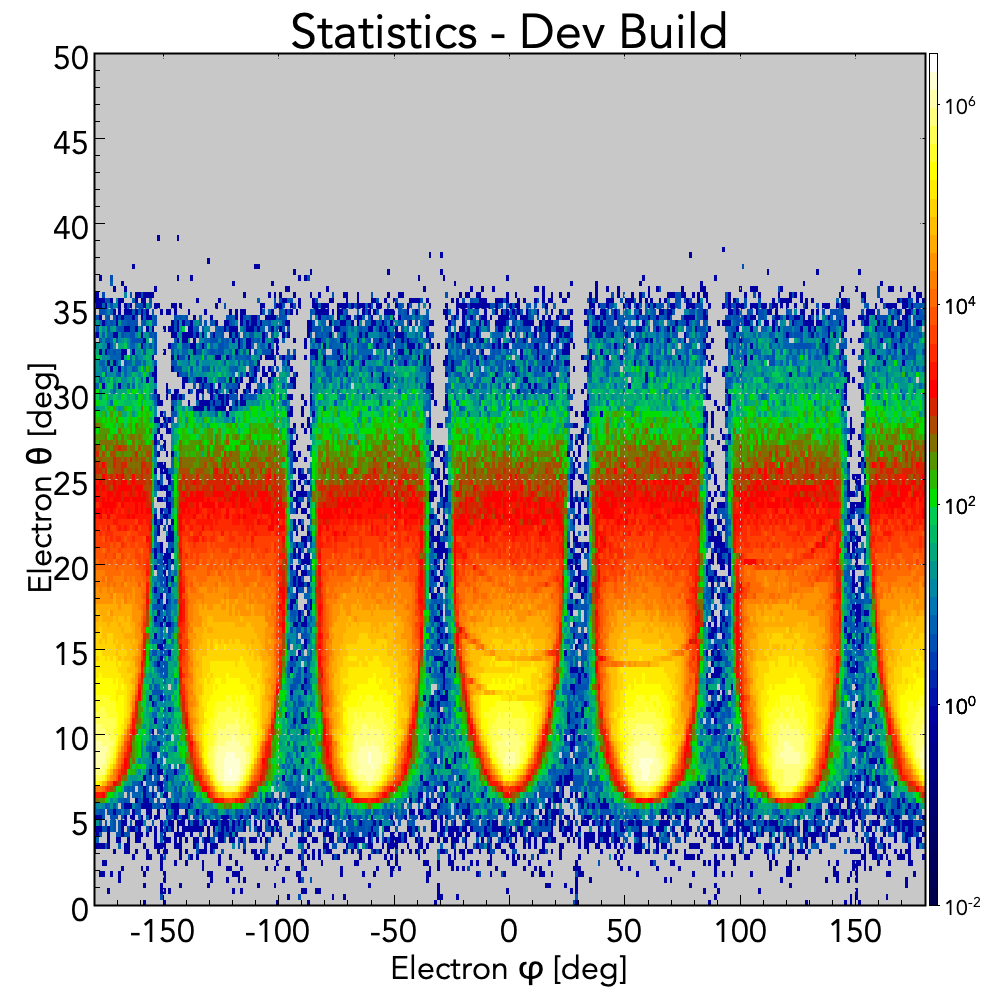
\includegraphics[width=1.0\linewidth,trim={0.0cm 0.0cm 0.0cm 1.67cm},clip]{images/statistics_Theta_Phi_Dev_Build_NO_HOLES.png}
    \caption{Distribution of statistics in all 6 sectors.}
    \label{fig:statistics_Theta_Phi_Dev_Build_NO_HOLES}
\end{figure}

We also note that in cases when the electrons cross the mirror close to its edges (at approximately at 5$^\circ$ and 35$^\circ$) one should expect unavoidable losses in the signal strength: some part of the Cherenkov light just passes by the mirror. As far as the internal borders between adjacent mirrors are concerned, there are similar losses that take place and are finally partially compensated due to the complete azimuthal symmetry of the detector, see Fig.~\ref{fig:avgNPE_Theta_Phi_Dev_Build-2_NO_HOLES}. The width of that area along internal boundaries that is deformed in the direction normal to the mirror face due to the shrinkage of the glue is estimated between $\sim$5 to $\sim$10 mm. This area includes the technological zone ~0.5 mm of width that is not reflecting the light at all. As a result these regions (width up to $\sim$10 mm) along internal boundaries between mirror facets defuse the light impinging the area, and therefore the signal strength is reduced. this edge effect is normal for the given design of the detector.



\section{M{\o}ller Polarimeter}
\label{mollerpol}

Determination of the electron beam polarization is done in Hall B using a coincidence M{\o}ller polarimeter.  The polarimeter is based 
on ${\vec e} + {\vec e}\rightarrow e + e$  elastic scattering (M{\o}ller scattering).  A detailed description of M{\o}ller scattering is presented 
in Ref.~\cite{Wagner:1990sn}.  

For a longitudinally polarized electron beam incident on a longitudinally polarized electron target, the 
center-of-momentum (CM) frame cross section is given by \cite{moller32,kresnin57}
\begin{equation}
\label{eq-csec}
 {{d\sigma}\over{d\Omega}}=
  {{d\sigma_0}\over{d\Omega}}\left(1+P_BA_{zz}P_T\right),
\end{equation}
where $d\sigma_0/d\Omega$ is the unpolarized cross section, $P_B$ and $P_T$ are the longitudinal components of the beam and target polarization, respectively, and $A_{zz}$ is the analyzing power.
The unpolarized cross section and analyzing power can be precisely calculated through QED, which gives
%
\begin{equation}
\label{eq-csecCM}
	\frac{d\sigma_0}{d\Omega}=\left(\frac{\alpha\left(3+\cos^2\theta_{CM}\right)}
						{2m_e\gamma\sin^2\theta_{cm}}\right)^2,
\end{equation}
%
and 
\begin{equation}
\label{eq-Azz}
	A_{zz}=-\frac{\left(7+\cos\theta_{CM}\right)\sin^2\theta_{CM}}{\left(3+\cos^2\theta_{CM}\right)^2},
\end{equation}
%
where $\alpha$ is the fine structure constant, $\theta_{CM}$ is the center of momentum scattering angle, $m_e$ is the electron mass, and
$\gamma=\sqrt{\left(E+m_e\right)/2m_e}$ with $E$ the lab energy of the incident electron.
From the above formulas, one sees that $A_{zz}$ has a maximum magnitude of $7/9$ at $\theta_{CM}=90^\circ$, which is the central scattering
angle for our polarimeter.

Forming the beam-helicity-dependent asymmetry gives
\begin{equation}
\label{eq-asymm}
	A=\frac{\frac{d\sigma}{d\Omega}_+-\frac{d\sigma}{d\Omega}_-}{\frac{d\sigma}{d\Omega}_++\frac{d\sigma}{d\Omega}_-}
	=A_{zz}\left(\theta_{CM}\right)P_B^zP_T^z,
\end{equation}
where the $\pm$ refers to cases where the beam helicity and the target polarization are aligned or anti-aligned.
The asymmetry can be measured from the yields according to
%
\begin{equation}
\label{eq-asymm-meas}
	A=\frac{N_+-N_-}{N_++N_-}=\langle A_{zz}\rangle P_B^zP_T^z,
\end{equation}
%
where $\langle A_{zz}\rangle$ is the effective analyzing power corrected for the finite-angle acceptance of the polarimeter and atomic-electron
motion (also known as the Levchuk effect \cite{levchuk94}).


The CLAS12 M{\o}ller polarimeter detects the scattered electrons in coincidence near $\theta_{CM}=90^\circ$, the peak of $A_{zz}$.  
The coincidence method has the advantage, as compared to 
single-arm M{\o}ller polarimetry, of producing a clean data set without having to do 
energy-dependent background subtractions (see, for example Ref.~\cite{arrington92}). Accidental background rates are typically less than
$10\%$ of the real coincident rate for our polarimeter. The accidental rate is measured and included as a correction.

\subsection{Polarimeter Design}
\label{sec-PolDesign}

The layout for the polarimeter is shown in Fig.~\ref{fig-PolLayout}. The essential elements of the polarimeter include a polarized target 
system, a pair of quadrupole magnets both operated in a dispersive mode to separate the scattered electrons for the unscattered  
beam electrons, a pair of detectors, and lead shielding between the second quadrupole and the detectors to reduce 
background.  The detectors consist of scintillating fibers packed with lead powder to form a 15.6-cm wide, 9.0-cm high, and 25-cm deep 
block with a light guide and read out with a PMT. The detectors are surrounded by 
lead bricks with a scattered-particle aperture of 7.62 cm in the horizontal direction and 5.0 cm in the vertical direction.
The locations of the quadrupoles and detectors along with the quadrupole fields were determined by simulations of the layout. The 
locations and fields were adjusted in the simulation so that $\theta_{CM}=90^\circ\pm (4^\circ-4.5^\circ)$.

\begin{figure*}[hbtp]
 \begin{center}
  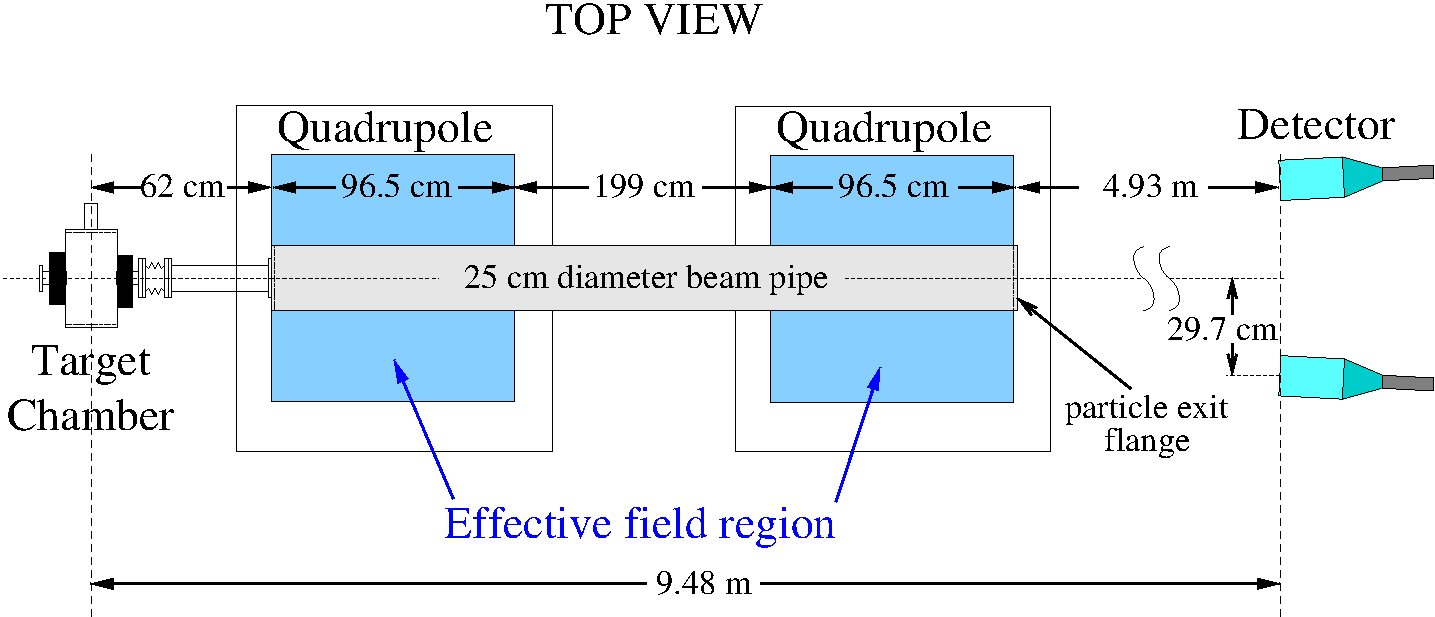
\includegraphics[width=\textwidth]{MPLayout.pdf}
 \end{center}
 \caption[]{Layout of the CLAS12 M{\o}ller polarimeter. Detector shielding is not shown.}
 \label{fig-PolLayout}
\end{figure*}


\subsubsection{Polarimeter Target}
\label{sec-PolTgt}

The target system has a pair of 25-$\mu$m-thick permendur foils on a remotely controlled insertion table housed in a vacuum 
chamber, as shown in Fig.~\ref{fig-MPtgt}. Permendur is an iron-cobalt alloy (49\% Fe, 49\% Co, 2\% Va) that has a saturated polarization
of approximately 8\% along the plane of the foil when subjected to a magnetic field of greater than about 40 G. To create a longitudinally 
polarized target, the plane of a foil is 
oriented at $\pm 20^\circ$ relative to the beamline and subjected to a longitudinal magnetic holding field produced by a pair of Helmholtz 
coils on either side of the target chamber. Since only the longitudinal component of the polarization contributes to the
measured asymmetry, the target polarization used in Eq.~\ref{eq-asymm-meas} is $P_T^z=P_T\cos 20^\circ$. 

\begin{figure}[hbtp]
 \begin{center}
  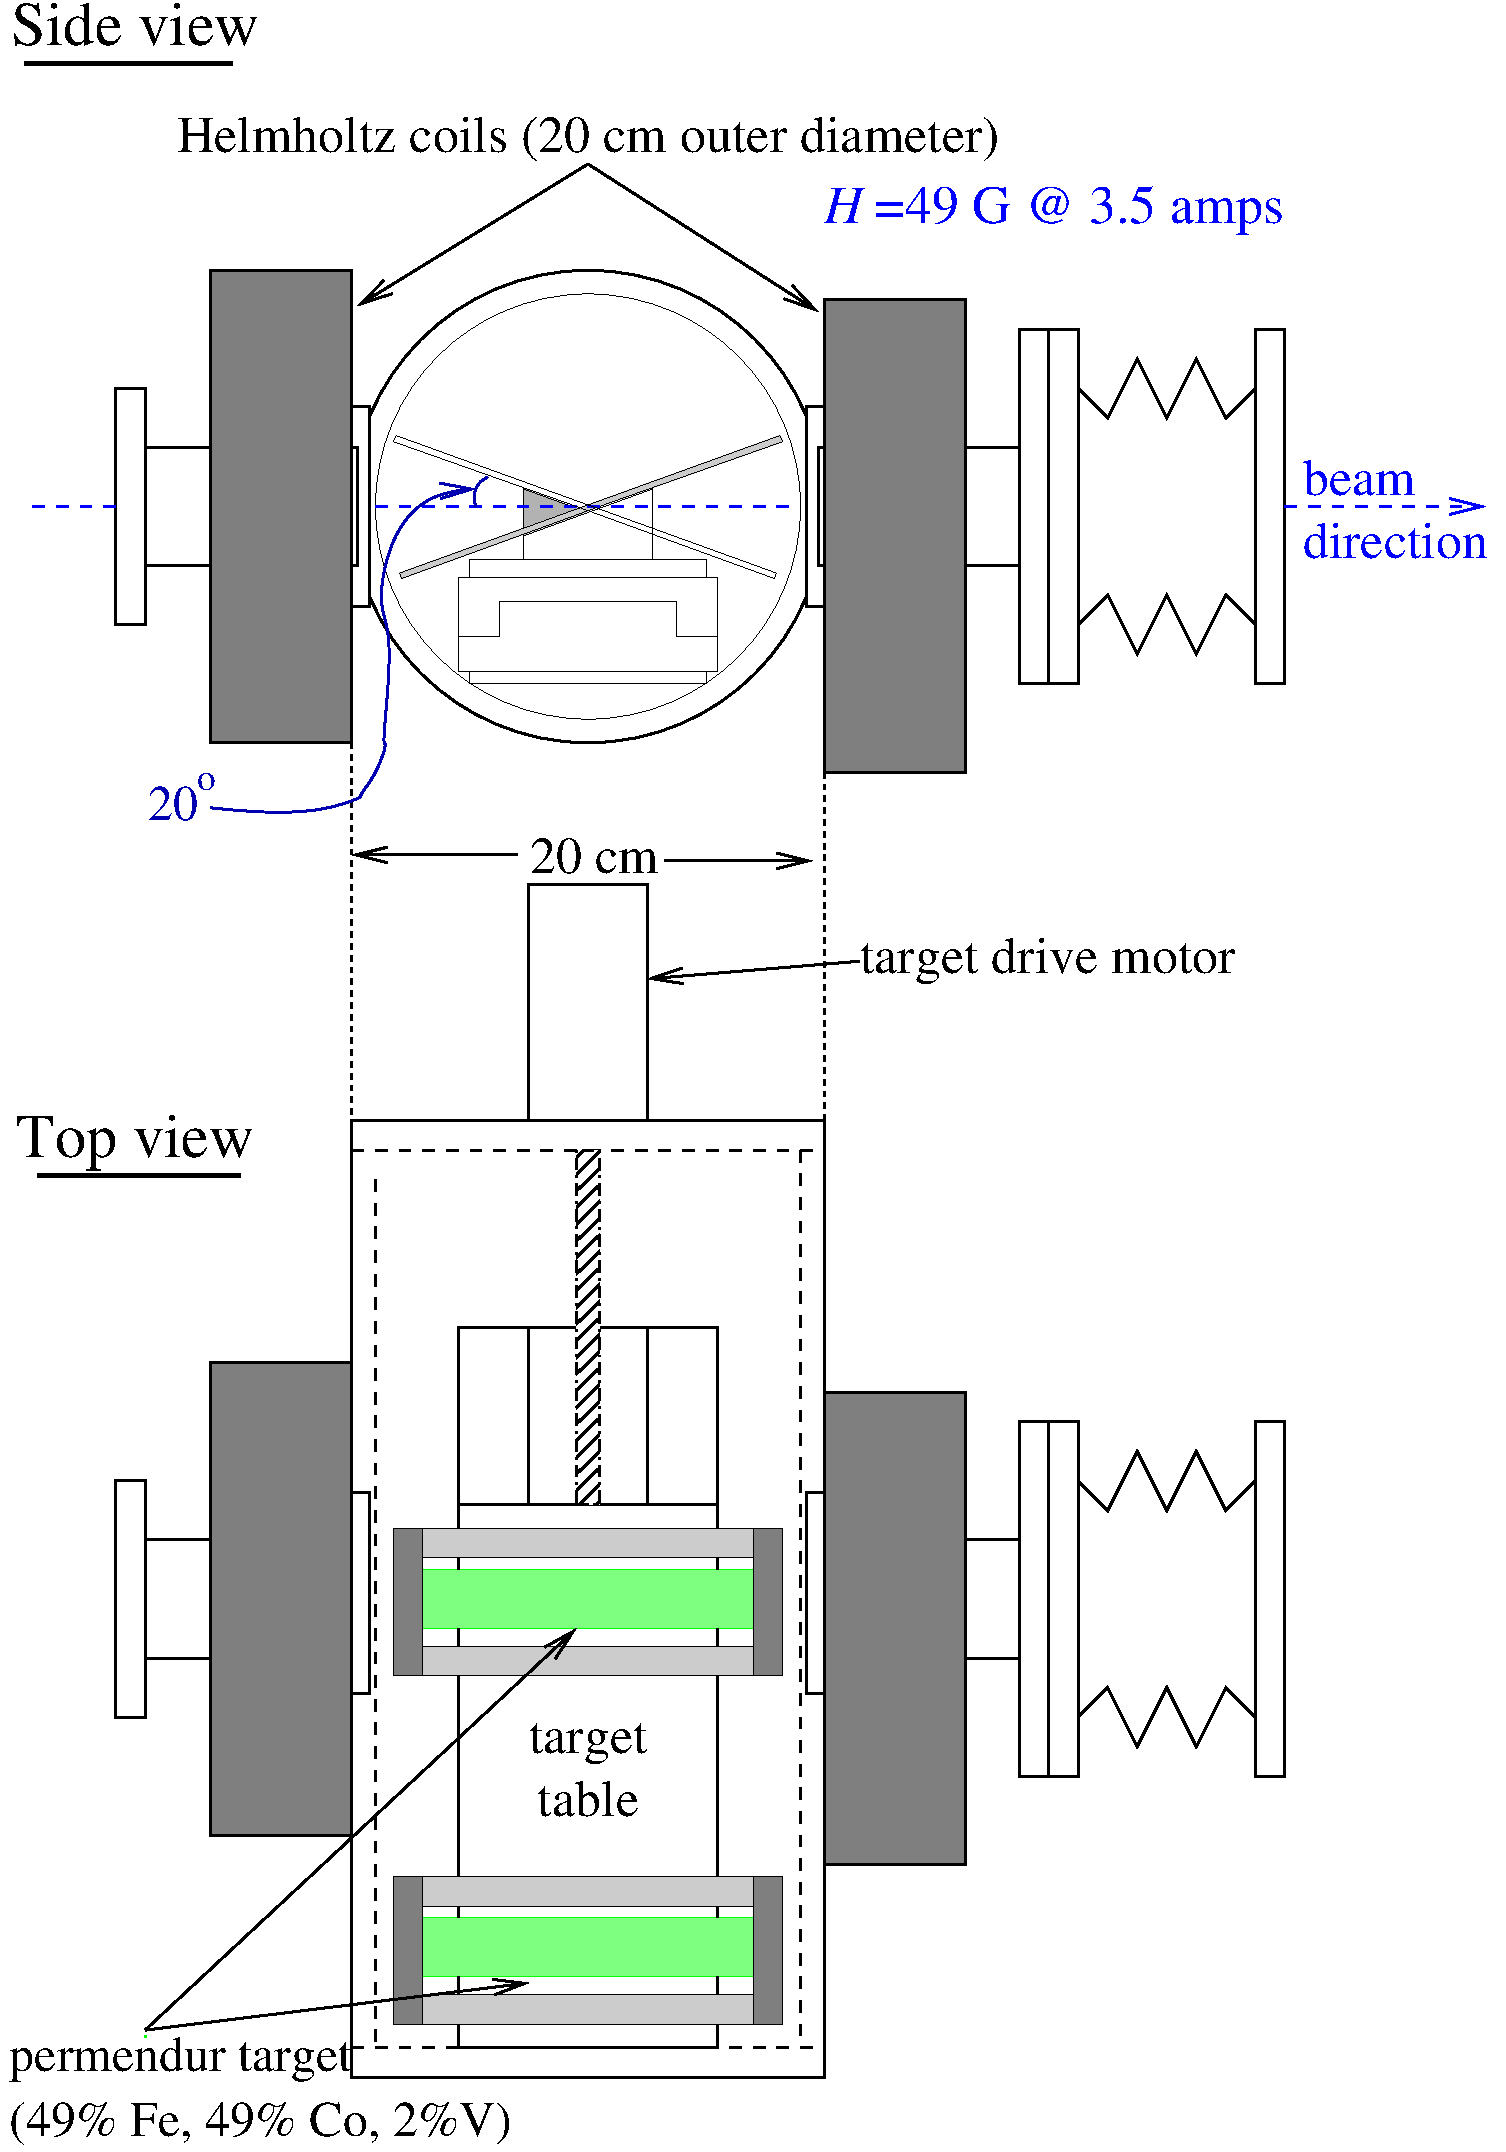
\includegraphics[width=0.5\textwidth]{MPtgt.pdf}
 \end{center}
	 \caption[]{Layout of the CLAS12 M{\o}ller polarimeter target chamber. Shown with the beam-left target inserted.}
 \label{fig-MPtgt}
\end{figure}

The polarization of the permendur target is related to the magnetization, $M$, of the foil by \cite{Band:1997ee} 
%
\begin{equation}
\label{eq-M2Pt2}
	P_T=M\left(4.546\times 10^{-5}\pm 2.9\times 10^{-7}\right),
\end{equation}
%
where $M$ is measured in units of G. The foil magnetization is measured in a separate setup consisting of a solenoid coil used to produce 
the magnetizing field, $H$, into which the target foil is placed and a pickup coil that is located at the center of the foil. A fixed current is 
applied to the solenoid to polarize the target. The direction of the current is then flipped over a time period of ~0.15 s leading to an 
induced voltage across the pickup coil. A typical pickup-coil signal is shown in Fig.~\ref{fig-TPolMeas}, which was measured with a 
digital storage oscilloscope. The flat part of this signal (highlighted by the black constant fit) corresponds to the changing applied field while 
the narrow peak in the middle of the signal results from the change in the target foil magnetization. Applying Faraday's law to the flat part of 
the signal (using the fit to interpolate under the peak) yields
%
\begin{equation}
\label{eq-H}
	\int_H  Vdt=2HN_T \langle A_{\rm coil}\rangle\rightarrow H=\frac{\int_H Vdt}{2N_T\langle A_{\rm coil}\rangle} ,
\end{equation}
%
where $\int_H Vdt$ is the area under the pickup coil signal excluding the peak, $N_T$ is the number of turns in the pickup coil, and 
$\langle A_{\rm coil}\rangle$ is the average cross-sectional area of the pickup coil.
Since the magnetization is related to the total field, $B$, and the applied field, $H$, through $4\pi M=B-H$, then
%
\begin{equation}
\label{eq-M}
	M=B-H=\frac{1}{4\pi}H\left(\frac{\int_{\rm total} Vdt-\int_HVdt}{\int_HVdt}\right),
\end{equation}
%
where $\int_{\rm total} Vdt$ is the total area of the signal. Figure~\ref{fig-PSat} shows a typical saturation curve for the target, i.e. how 
the target polarization depends on the applied field. Measurements were done with two different pickup coils with the difference between 
the two results indicating the systematic uncertainty associated with knowledge of the coil geometry. For this foil, the polarization saturates 
at a value of $7.31\pm 0.08$\%, where the uncertainty is a combination of the statistical uncertainties from the linear fits of the saturation
region of the curves and the variation between the two measurements. Additional uncertainties associated with converting from $M$ to $P_T$ 
(Eq.~\ref{eq-M2Pt2}), the uncertainty from estimated variations in the target material thickness, and the uncertainty in the target angle relative
to the beam lead to an overall uncertainty of $0.13\%$ and a total relative uncertainty $\delta P_T^z/P_T^z=0.018$.



\begin{figure}[ht]
 \begin{center}
  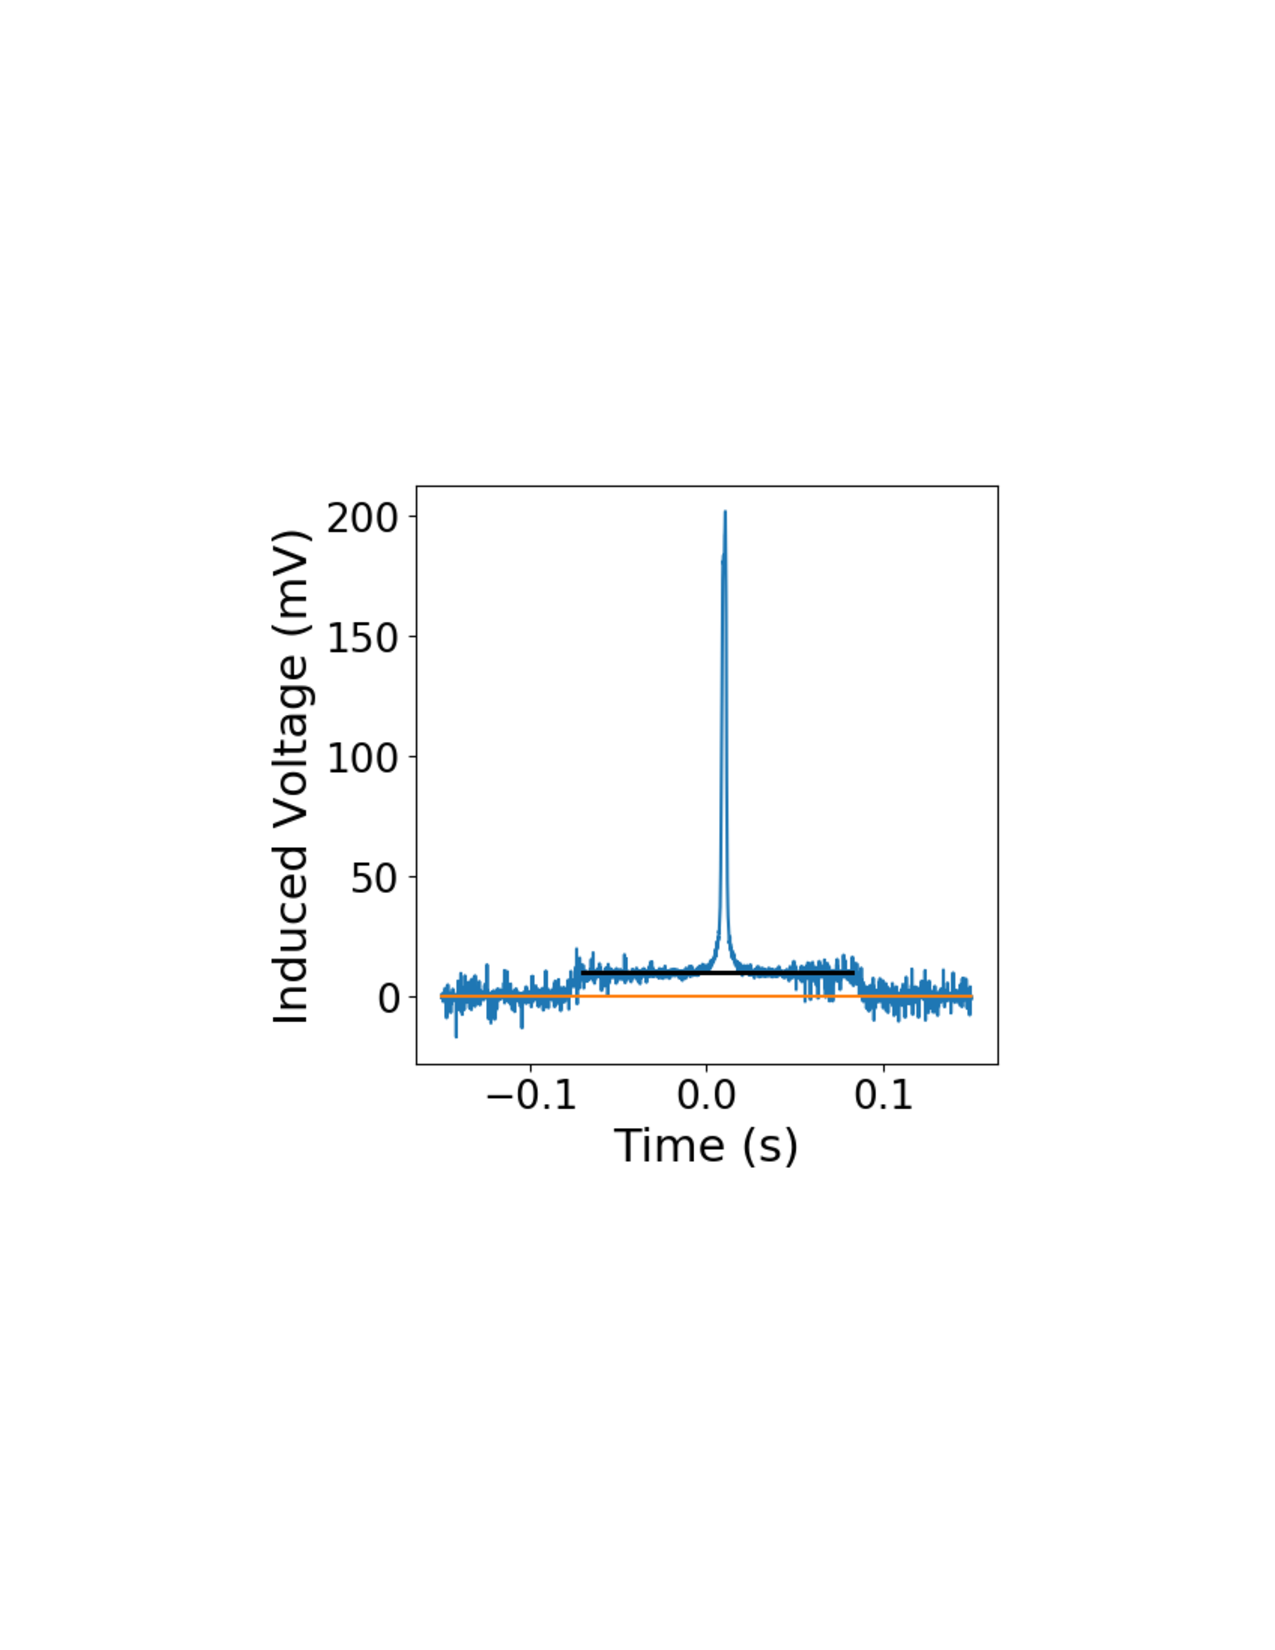
\includegraphics[width=0.45\textwidth]{11Vtgtdata.pdf}
 \end{center}
 \caption{Target pickup coil signal showing induced voltage as a function of time.  The flat part of the signal (fit with black line) corresponds 
 	to the changing applied Helmholtz field, $H$, while the sharp peak near the middle corresponds to the flip in the target magnetization.}
 \label{fig-TPolMeas}
\end{figure}

\begin{figure}[ht]
 \begin{center}
  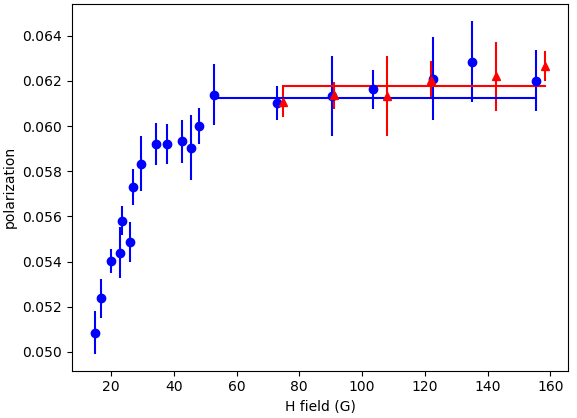
\includegraphics[width=0.45\textwidth]{PvsH0.png}
 \end{center}
	\caption{Target polarization vs.~applied magnetic field, $H$, measured with two different pickup coils. A constant fit to the flat part 
	of the curves yields values of $7.35\pm 0.04$\% for coil 1 (red diamonds) and $7.24\pm 0.05$\% for coil 2 (blue dots).} 
 \label{fig-PSat}
\end{figure}

\subsection{Analyzing Power Corrections and Uncertainties}
\label{sec-PolCor}

Simulations have been performed to estimate effects due to atomic motion of the electrons and to estimate uncertainties associated with 
the polarimeter geometry. The simulation begins by randomly selecting scattering angles $\theta_{CM}$ and $\phi_{CM}$ and then transports
the scattered electrons through the magnets and towards the detectors. For events in which both electrons hit the detectors we determine an 
average analyzing power, $\langle A_{zz}\rangle$. The motion of the atomic electrons has been included in the simulation according to
Ref.~\cite{levchuk94}. Figure~\ref{fig-Azz} shows $\langle A_{zz}\rangle$ as a function of beam energy both with (orange) and without 
(blue) atomic-electron motion included in the simulation. The green curve is a fit to the points 
$\langle A_{zz}\rangle= -0.777123+(2.9249\times 10^{-3})/E$. 
The estimated relative uncertainty is $<0.01$\% and was determined by looking at variations in $\langle A_{zz}\rangle$ for reasonable 
variations in the geometry (locations of quadrupoles and detectors) and magnetic fields.
\begin{figure}[ht]
 \begin{center}
  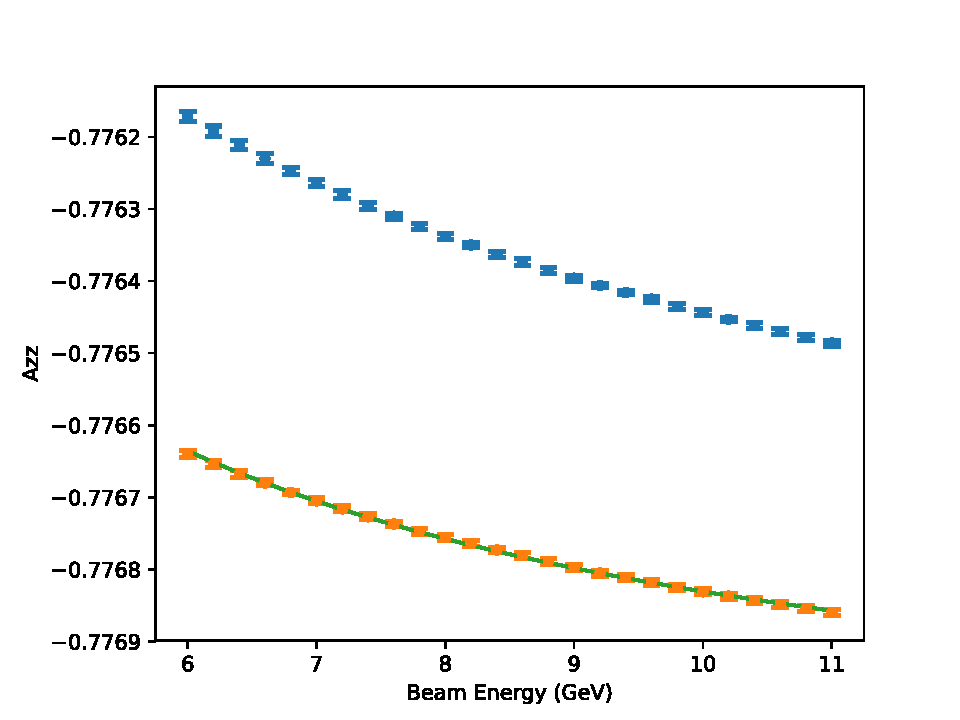
\includegraphics[width=0.45\textwidth]{Azz.pdf}
 \end{center}
	\caption{Average analyzing power $\langle A_{zz}\rangle$ as a function of beam energy from simulation. The orange/blue points 
	include/exclude motion of the atomic electrons. The error bars are statistical only. The green curve on the orange points is a fit 
	given in the text.}
 \label{fig-Azz}
\end{figure}


%but has negligible effect due to a relatively large angular acceptance ($\delta\theta^{lab}/\theta^{lab}\approx0.14$). 


%\subsection{Spin Dance}
\subsection{Beam polarization measurements}
\label{sec-SpinDance}

Beam polarization measurements are usually done on a weekly basis or after changes to the accelerator configuration.  The shift personnel
use what is in essence a push-button GUI interface shown in Fig.~\ref{fig:mollergui}. The user selects which target to use (left or right) and the
Helmholtz coil polarity. The settings for the quadrupoles are automatically calculated based upon the beam energy. Individual M{\o}ller runs
are usually done for both targets with a statistical precision of $\pm 1.5$\%, which is slightly smaller than the total systematic uncertainty. 
The underlying software calculates the beam polarization using the beam-helicity-gated true and accidental coincidence rates from 
the M{\o}ller detectors along with the beam-helicity related charge asymmetry measured using the SLM. 
At the end of a M{\o}ller run the beam polarization is stored in the database and displayed in the GUI, as seen in the upper right quadrant 
of  Fig.~\ref{fig:mollergui}. 

\begin{figure}[ht]
\begin{center}
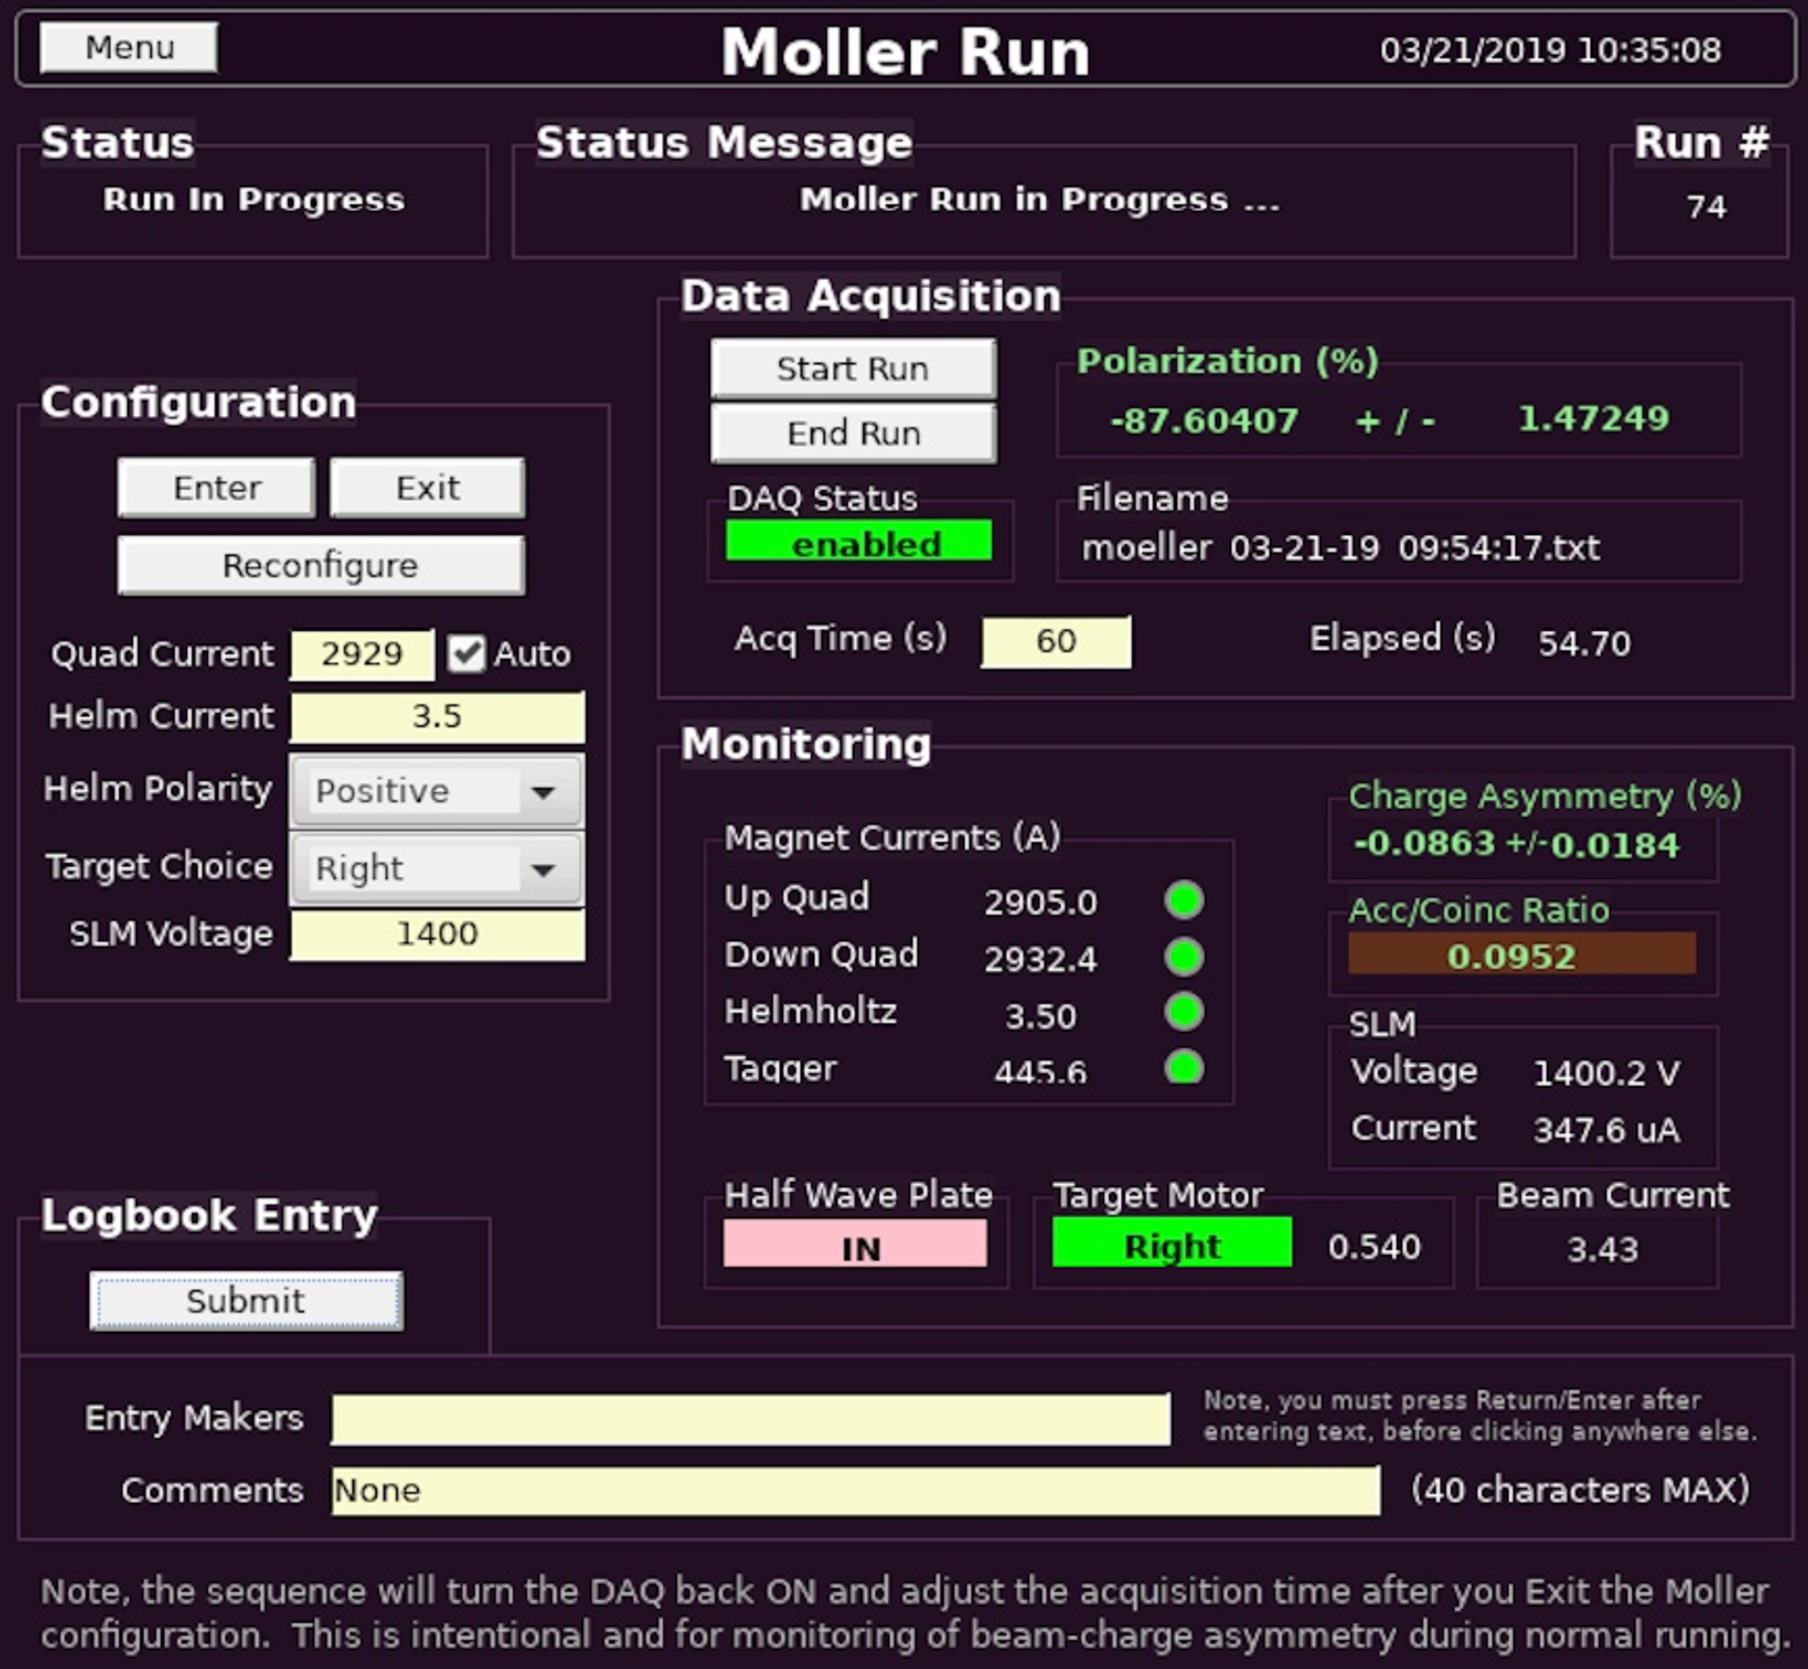
\includegraphics[width=0.475\textwidth]{moller_gui.pdf}
	\caption{Graphical user interface for M{\o}ller polarimeter operation.}
\label{fig:mollergui}
\end{center}
\end{figure}

Results of beam polarization measurements taken during the fall 2018 run period are shown in Fig.~\ref{fig:molrga}.
There are two distinct regions of beam polarization with average polarizations of $85.95\% ~\pm ~1.29\%$ and $89.22\%~\pm~2.51\%$. 
These two regions differ by settings of the angle, $\theta_W$ of the Wien filter in the injector. The initial setting of the Wien-filter angle was 
set to maximize the beam polarization in Hall B and is based on a calculation of the electron spin precession in the accelerator. 
However, the polarization in the early part of the running period fell below the expected maximum of about 90\%, which was measured 
at the injector by a Mott polarimeter, indicating an incorrectly calculated $\theta_W$ . In order to find the optimum value of $\theta_W$, 
two more M{\o}ller measurements of the beam polarization in Hall-B were performed at $\theta_W=25^\circ$ and $70^\circ$.  
The result of these measurements along with the average at $40^\circ$ are shown in Fig.~\ref{fig:sdance}. Fitting these three points 
with a function of $a\cos\left(\theta_W-b\right)$ (dashed curve), where $a$ and $b$ are fit parameters,  shows that the maximum
 polarization of about 90\% in Hall B occurs for $\theta_W\approx 40^\circ$.
 
\begin{figure}[ht]
\begin{center}
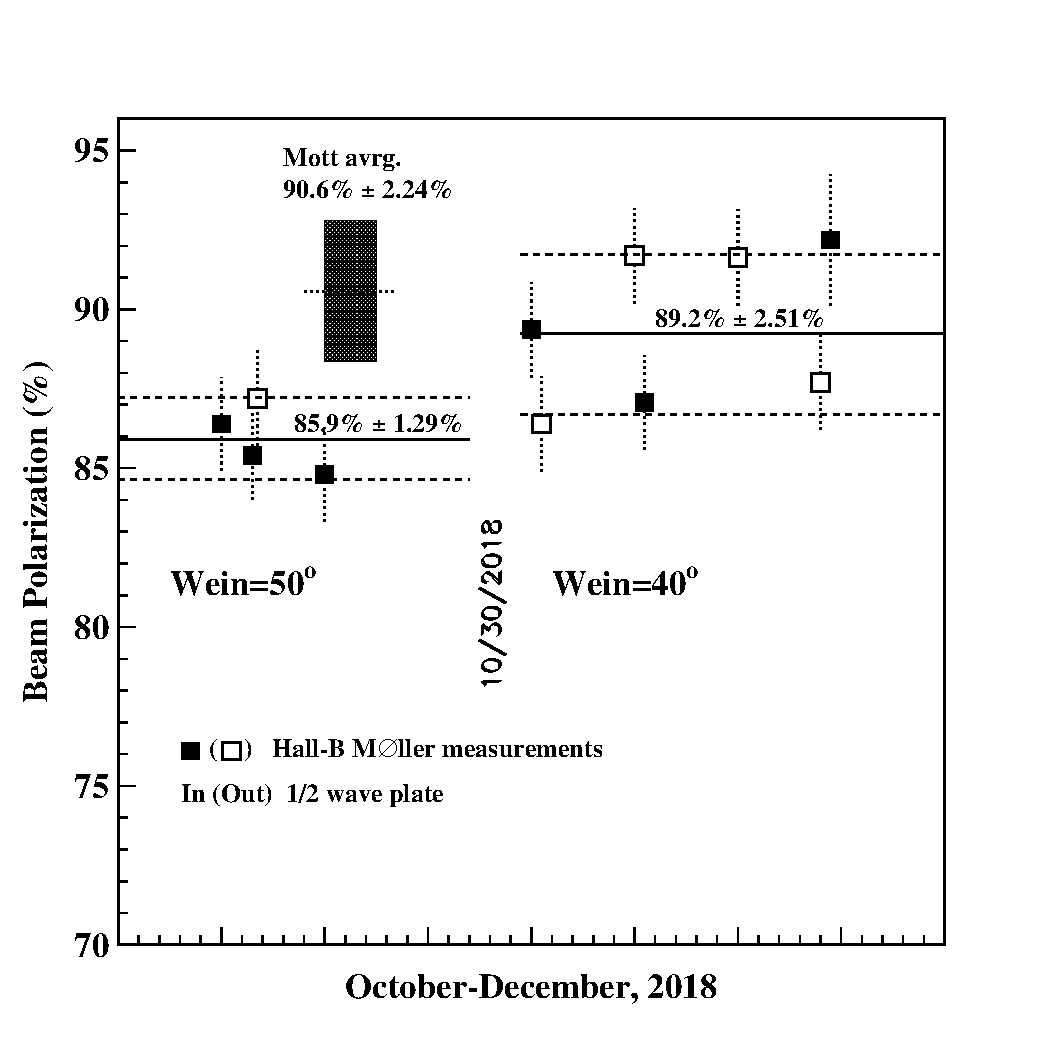
\includegraphics[width=0.5\textwidth]{Moller-RGA-2018.pdf}
	\caption{Beam polarization measured in Hall B during the fall 2018 running period. Prior to October 30 the measurements from the 
	Hall-B polarimeter (squares) averaged to $85.9\%\pm1.2\%$ (stat.), which is lower than the expected 90\% from the injector Mott 
	measurements (triangles). After the optimizing the Wien-filter angle the average polarization measured in Hall B was measured 
	to be $89.2\%\pm2.5\%$ (stat.). Filled and open symbols correspond to measurements made with and without a half-wave plate. Error bars
	are statistical only.}
\label{fig:molrga}
\end{center}
\end{figure}

\begin{figure}[ht]
\begin{center}
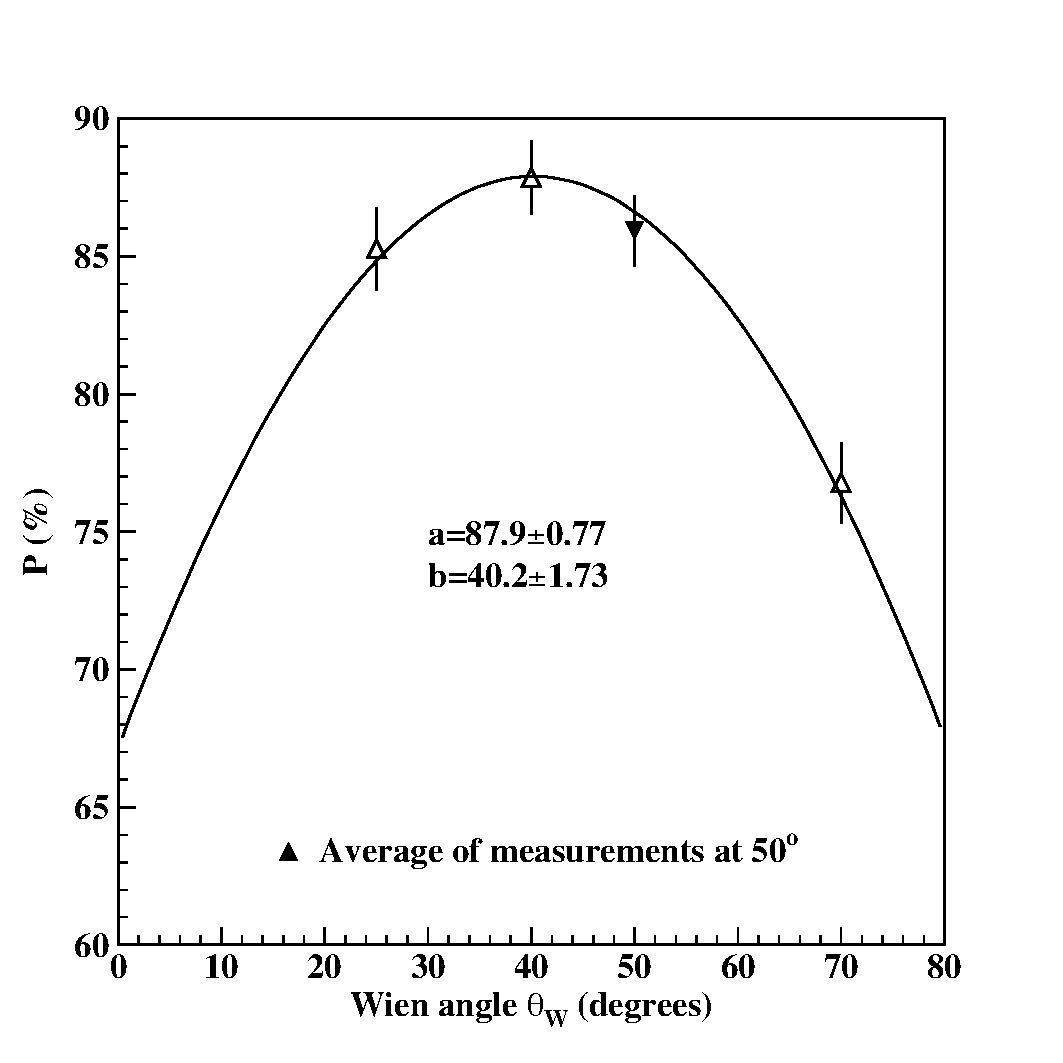
\includegraphics[width=0.5\textwidth]{Hall-B_fall_spin_dance.pdf}
	\caption{Beam polarization measurements at three different Wien angle settings taken during the fall 2018 run period.  The dashed 
	curve is the cosine-function fit to the data points. The filled point is the average over all measurements with the angle set to $50^\circ$ 
	and the open points are from single measurements. Error bars are statistical only. }
\label{fig:sdance}
\end{center}
\end{figure}

Figure~\ref{fig:molrga} has two sets of Hall-B polarimeter measurements done with and without a half-wave plate. The half-wave
plate rotates the electron spin by $180^\circ$. The measurements with and without the the half-wave plate agree within statistical
uncertainties. 



\section{Summary}

The first CLAS12 experiment in 2018 took data successfully at three beam energies; 10.6~GeV, 6.4~GeV, and
2.2~GeV with a liquid-hydrogen target. High quality beam was delivered with a beam size of $< 200$~$\mu$m
and a beam halo as small as 10$^{-4}$ at $5\sigma$ away from the core. The beam position was maintained within
$\sim$200~$\mu$m throughout the run  by the beam feedback system and the fast shutdown system worked in
protecting the CLAS12 detectors from errant beam exposure. With typical M{\o}ller polarimeter runs, the beam
polarization can be measured to an absolute precision of $\sim$2.5\%. 

\section{Acknowledgements}

The authors are grateful for the outstanding efforts by the staff of the Accelerator Division and the Hall~B
Engineering Group at Jefferson Lab during the installation and running of the experiment. We also thank the
CLAS12 Collaboration for manning shifts and taking high quality data. This material is based upon work supported
by the U.S. Department of Energy, Office of Science, Office of Nuclear Physics under contract
DE-AC05-06OR23177 and by the Italian Instituto Nazionale di Fisica Nucleare.

%% The Appendices part is started with the command \appendix;
%% appendix sections are then done as normal sections
%% \appendix

%% \section{}
%% \label{}

%% References
%%
%% Following citation commands can be used in the body text:
%% Usage of \cite is as follows:
%%   \cite{key}          ==>>  [#]
%%   \cite[chap. 2]{key} ==>>  [#, chap. 2]
%%   \citet{key}         ==>>  Author [#]

%% References with bibTeX database:

%\bibliographystyle{model1-num-names}
\bibliographystyle{elsarticle-num}
\bibliography{beamline_nim}
%\bibliography{<your-bib-database>}

%% Authors are advised to submit their bibtex database files. They are
%% requested to list a bibtex style file in the manuscript if they do
%% not want to use model1-num-names.bst.

%% References without bibTeX database:

\end{document}

%%
%% End of file `elsarticle-template-1-num.tex'.
